\documentclass[12pt,twoside,notitlepage]{report}
\newcommand{\fxch}{FixCache}
\newcommand{\etal}{\textit{et al.}}
\usepackage{a4}
\usepackage{verbatim}
\usepackage{amsmath}
\usepackage{color}
\usepackage[T1]{fontenc}
\usepackage[dvipsnames]{xcolor}
\usepackage{listings}
\usepackage{enumitem}
\usepackage[boxed]{algorithm2e}
\usepackage{fixltx2e}


\usepackage{graphicx}
\usepackage[labelfont=bf]{caption}
\usepackage{wrapfig}
\usepackage[rightcaption]{sidecap}
\usepackage[parfill]{parskip}
\usepackage{pdfpages}


\makeatletter
\setlength{\@fptop}{0pt}
\makeatother
\graphicspath{ {figs/} }
\title{Cached Bug Prediction for Python repositories on GitHub}
\author{Tamas Sztanka-Toth \\ ts579@cam.ac.uk}
\raggedbottom                           % try to avoid widows and orphans
\sloppy
\clubpenalty1000%
\widowpenalty1000%

\addtolength{\oddsidemargin}{6mm}       % adjust margins
\addtolength{\evensidemargin}{-8mm}

\renewcommand{\baselinestretch}{1.1}    % adjust line spacing to make
                                        % more readable

\begin{document}

\setcounter{page}{1}
\pagenumbering{roman}
\pagestyle{plain}
\bibliographystyle{unsrt}      % just to make sure before the page numbering
                        % is changed



\pagestyle{empty}

\hfill{\LARGE \bf Tamas Sztanka-Toth}

\vspace*{60mm}
\begin{center}
\Huge
{\bf Cached Bug Prediction for Python repositories on GitHub} \\
\vspace*{5mm}
Computer Science Tripos - Part II \\
\vspace*{5mm}
Homerton College \\
\vspace*{5mm}
\today  % today's date
\end{center}

\cleardoublepage

%%%%%%%%%%%%%%%%%%%%%%%%%%%%%%%%%%%%%%%%%%%%%%%%%%%%%%%%%%%%%%%%%%%%%%%%%%%%%%
% Proforma, table of contents and list of figures

\setcounter{page}{1}
\pagenumbering{roman}
\pagestyle{plain}

\chapter*{Proforma}

{\large
\begin{tabular}{ll}
Name:               & \bf Tamas Sztanka-Toth                       \\
College:            & \bf Homerton College                     \\
Project Title:      & \bf Cached Bug Prediction for Python\\ 						& \bf repositories on GitHub \\
Examination:        & \bf Computer Science Tripos - Part II, 2016        \\
Word Count:         & \bf 11987\footnotemark[1]				 \\
Project Originator: & Advait Sarkar                \\
Supervisor:         & Advait Sarkar                    \\ 
\end{tabular}
}
\footnotetext[1]{This word count was computed
by {\tt detex diss.tex | tr -cd '0-9A-Za-z $\tt\backslash$n' | wc -w}
}
\stepcounter{footnote}
\section*{Original Aims of the Project}
To implement the \fxch{} bug prediction algorithm in Python for Git repositories.  Once the algorithm is implemented, analyse and evaluate it on five different open-source Python projects on GitHub and compare these results with the ones found by the original authors who analysed Java and C/C++ projects. Finally, implement a new evaluation technique for \fxch{} and evaluate the algorithm with this new method.
\clearpage
\section*{Work Completed}
The core algorithm, together with other supporting modules was implemented on time. It was tested and analysed with the repositories outlined in the project proposal, and results were compared with previous research findings. Lastly, the performance of \fxch{} was measured using a new evaluation technique.

\section*{Special Difficulties}
None.
 
\newpage
\section*{Declaration}

I, Tamas Sztanka-Toth of Homerton College, being a candidate for Part II of the Computer
Science Tripos, hereby declare
that this dissertation and the work described in it are my own work,
unaided except as may be specified below, and that the dissertation
does not contain material that has already been used to any substantial
extent for a comparable purpose.

\bigskip
\leftline{Signed }

\medskip
\leftline{Date }

\cleardoublepage

\tableofcontents

\listoffigures

\newpage
\section*{Acknowledgments}
I would like to thank my supervisor, Advait Sarkar, for his guidance and advises throughout the project. This work would have been much harder without his valuable and helpful feedback, comments and suggestions.

%%%%%%%%%%%%%%%%%%%%%%%%%%%%%%%%%%%%%%%%%%%%%%%%%%%%%%%%%%%%%%%%%%%%%%%
% now for the chapters

\cleardoublepage        % just to make sure before the page numbering
                        % is changed
\setcounter{page}{1}
\pagenumbering{arabic}
\pagestyle{headings}
\chapter{Introduction}
This dissertation describes and analyses \fxch{} \cite{FixCache}, a bug prediction approach which uses  the version history of a repository to identify bug-prone files. First it will discuss what preparatory work was done before the implementation, in order to acquire the necessary background knowledge. Then, it will show the process of implementing this algorithm in Python, for open-source Python repositories on GitHub.

The implemented algorithm is then analysed and evaluated against \textit{hit-rate}, a metric introduced by Kim \etal{} \cite{FixCache}. Although results indicated that the repositories in this dissertation performed slightly poorer than the projects which Kim \etal{} looked at, it will be deduced that the algorithm indeed works for Python open-source repositories on GitHub.

In addition to evaluating against hit-rate, a new evaluation technique is introduced. Using this method, it was found that \fxch{}'s performance is only high for a short period of time in the future, and that after that the performance drops by roughly 30-40\%.

This chapter will further talk about motivation behind the dissertation itself, and briefly describe the previous work done in the field of bug prediction.
\clearpage
\section{Motivation}
Testing and debugging has always been one of the most important parts of Software Development. Companies and developer teams spend a lot of time and effort when finding and fixing bugs prior to releasing a new version of a product.

As projects grow bigger every day, their complexity also increases, which further means that testing and modelling also becomes harder. As follows, developers have to write more complex unit-tests and debugging tools, which will cover a wider range of use cases.

However even with the most advanced testing tools and review techniques there still are bugs discovered only after deployment, and therefore bug prediction techniques have gained importance. These, as opposed to static paradigms (like unit-testing) will use data associated with a software (or its repository) to identify and predict bugs.

\section{Previous work}
There are several approaches to bug prediction to date, which can be put into two main categories: \textbf{Change-log approaches} and \textbf{Single-version approaches} \cite{5463279}. These approaches usually use different types of data for prediction (as seen in figure \ref{bug_prediction_data}), but ultimately all of them try to achieve the same result: to narrow down the set entities (files, classes, functions) to entities which are the most bug prone, that is they are most likely to contain a bug in the future.
\begin{figure}[h]
\vspace*{0.1in}
\hspace*{0.1\textwidth}
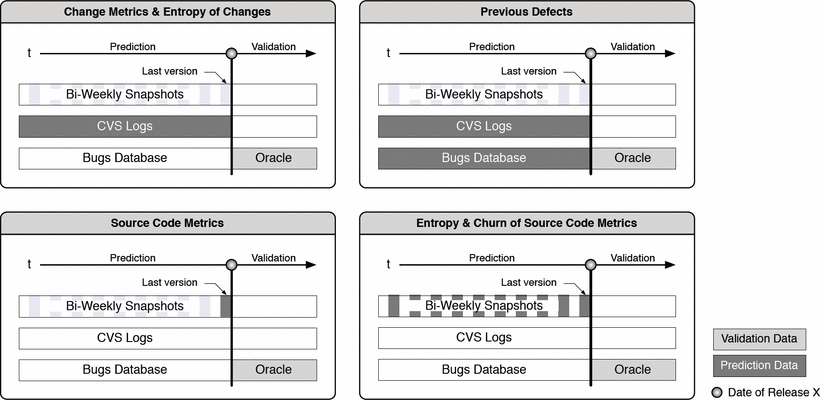
\includegraphics[width=0.8\textwidth]{bug_prediction_data.png}
\centering
\captionsetup{width=0.7\textwidth}

\caption[Examples of data that might be used by different bug prediction approaches]{Examples of data that might be used by different bug prediction approaches. Figure taken from D'Ambros \etal{} \cite{5463279}.}.
\label{bug_prediction_data}
\end{figure}

\paragraph{Single-version approaches}They use the current state of the repository and calculate variety of metrics  to predict faulty behavior. The most commonly used metric is the so-called Chidamber and Kremmer (CK) metrics suite\cite{295895}. It was proposed for Object-oriented programs (OOP), and it quantifies the state of a program using different data. For example, one metric is the \textit{Weighted Method Count per Class} (WMC): the sum of the \textit{complexities} of the methods in a class. The definition of the per method \textit{complexity} measure is left open by Chidamber and Kremmer, they only suggest it should be an additive property \cite{295895}.

There are several other OOP metrics used, which weren't suggested as a part of CK metrics. A simple example might be, the \textit{Lines Of Code} per file, or method (LOC).

These metrics are then used as a part of a bug prediction or bug-identification scheme. Several such schemes were proposed, for reference and examples one should look at the listings described by D'Ambros \textit{et al.} \cite{5463279}.

\paragraph{Change-log approaches}In contrast, the Change-log approaches look at how repositories evolved over time, and try to predict where the future defects will occur. For example Hassan's algorithm calculates the complexity of each change and calculates the entropy of these changes which then is used for bug prediction \cite{hassan}.

\fxch{} is also a change-log approach to bug prediction: the algorithm looks at the version history of a repository, it tries to identify more bug-prone entities. It was introduced by Kim \textit{et al.} in 2007, who implemented it for both files and methods \cite{FixCache}. These two approaches differ only in that the first looks at files while the second looks at methods as the basic entities the algorithm is ran on. This dissertation will only consider the file-based approach.

Since it's introduction, \fxch{} has been researched and tested heavily: Sadowski \etal{} analysed how the algorithm performs on files, and how does hit-rate perform over time \cite{Sadowski}. Rahman \etal{} compared the algorithm to other prediction techniques, and found it to be better than a naive prediction technique, but not significantly \cite{Bugcache}.
\clearpage
Previous implementations \cite{FixCache}\cite{Sadowski}, except one \cite{Bugcache} did not use Git \cite{TorvaldsGit} as their back-end Version Control System (VCS), but rather they used an alternative system such as Subversion (SVN) or CVS. These Version Control Systems differ in many aspects, which will be discussed more broadly in section \ref{section-Git}. Also, these implementations were solely ran on C/C++ and Java projects, hence my motivation to implement \fxch{} and run it on public Python repositories on GitHub.
\section{Resources and Terminology}
The \fxch{} implementation presented in this dissertation was tested, analysed and evaluated on a remote server machine, with two Intel Xeon E5-2620\footnote{http://ark.intel.com/products/64594/} processors with 64GB of RAM, running a Debian Linux.

\fxch{} can be implemented for two different entities: files and methods. The first will identify buggy files, while the second will identify buggy methods. As this dissertation discusses only \fxch{} implemented for files as entities, each time I use the word `entity' it refers to a file.

In Git `revision and `commit' are different notions: the first refers to a pointer by which one can reference a Git object (for instance a commit or a branch), whereas the second is used when talking about commit-objects. In this dissertation I will use them as synonyms, whenever I write `revision' I mean `commit'.
\cleardoublepage
\chapter{Preparation}
This chapter summarizes the work done before implementation: it first discusses \fxch{} and it's background; then it describes Git \cite{TorvaldsGit} software management system and how can it be used to implement \fxch{}. Finally, in this chapter will introduce a development tool used in this dissertation: GitPython, a Python library used to access Git repositories.
\section{Overview \fxch{}}
The algorithm itself is called \fxch{} as it uses a notion of a cache, which contains a fixed subset of files from a repository (fixed subset means that the size of our cache is limited, and constant for a single run). 

During one run, we go through all the commits in a repository, and at each commit we modify our cache so that at each point it contains the files which are believed to be more bug-prone than others. After the algorithm has completed, the files which ended-up in the cache are said to be more bug-prone, and they are the ones which are most likely to have bugs in the future \cite{FixCache}.
\clearpage
\begin{figure}[h]
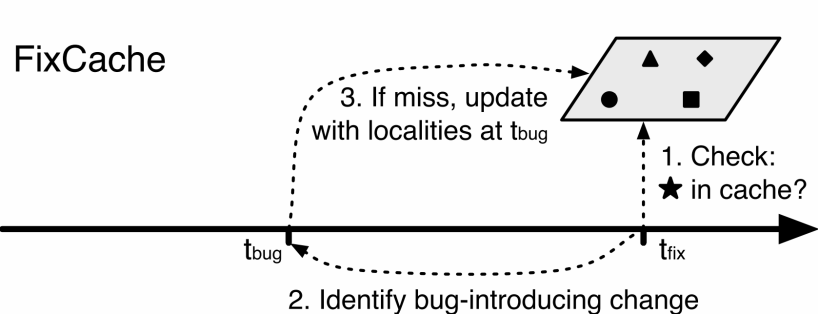
\includegraphics[width=0.6\textwidth]{fixcache_figure.png}
\centering
\captionsetup{width=0.6\textwidth}
\caption{Abstract view of how \fxch{} proceeds when a bug-introducing change is encountered.}.
\label{fixcache_figure}
\end{figure}
\subsection{Abstract view of the algorithm}
For a given repository, the algorithm works as follows:
\begin{enumerate}
	\item Pre-load the cache with initial files.
	\item For each commit $C$ in the repository, starting from the first commit:
	
	\item If $C$ is identified as a fixing-commit (a bug-fixing commit):
	\begin{enumerate}
	\item \label{lookup} For each file in $C$, we check if they are in the cache. If a file is in the cache, we record a hit; else we record a miss.
	\item For each file $F$ which was not in the cache, we identify the commits which introduced the bug(s) fixed by $C$. We take the closest files to $F$ at these bug-introducing commits, and put them into the cache.
	\end{enumerate}
	\item We put new-files and changed-files at $C$ into the cache.
	\item We remove the files from the cache, which were deleted at $C$.
\end{enumerate}

Figure \ref{fixcache_figure} shows how the algorithm proceeds at step 3, when we identify a fixing-commit.

So far, we only talked about adding files to the cache, but our cache has a limit of how many files it can store. To ensure that new files can be added, behind the scenes the algorithm should take care of cache pollution, and should remove files from the cache to make space for new arrivals.
\subsubsection*{Cache-replacement policies}
As the number of files in the cache (the cache-size) is fixed, we need to take out files from the cache if the cache is polluted. There exist different cache-replacement policies \cite{FixCache}:
\begin{itemize}
\item \textit{Least-recently-used (LRU)}: When removing files from the cache we first remove those which were used least-recently. That is we remove the files which were added/changed earlier in our commit history.
\item \textit{LRU weighted by number of changes (CHANGE)}: This approach will remove files which were changed the least, as the intuition is that more frequently used files are more bug-prone, so we want to keep them in the cache.
\item \textit{LRU weighted by number of faults}: This is similar to the approach before, the only difference is that instead of removing files with least changes it removes files with least faults.
\end{itemize}
In the implementation itself LRU has been used as it is the simplest, and there was no significant difference identified between the different replacement policies by neither of the previous implementations \cite{FixCache}\cite{Sadowski}\cite{Bugcache}.
\subsection{Hits, misses and hit-rate}
We only look-up the cache at the so-called bug-fixing commits (step \ref{lookup} in the abstract view). To flag a commit as a bug-fixing one, we use a set of regular expressions (which are discussed in more detail in section \ref{parsing}) to parse it's commit message. If a message matches any of our regular expressions, a bug-fixing commit is identified  (following the idea used in \cite{KimZim}).
Some examples of bug-fixing commit messages\footnote{All examples taken from identified commit-messages of facebook-sdk.git repository.}:
\begin{itemize}
\item \texttt{Simple json module import. Fixes \#106.}

\item \texttt{bugfix: changed key of id from user to id in the user dict stored in the session}
\item \texttt{Final fix for Python 2.6 tests.}
\item \texttt{PEP8 fixes. Make sure that code is compliant with pep8 1.3.3.}
\end{itemize}

At each bug-fixing commit, for each file involved in that commit, we make a look-up in the cache. If a file is already in the cache, we note a \textbf{hit}. Otherwise we score a \textbf{miss}.
\subsubsection*{Hit-rate}
Once we have the number of hits and misses, we can define \textbf{hit-rate}, as the ratio of hits over all look-ups, that is:
\vspace{0.2in}
\[
	\operatorname{hit-rate} = \frac{\#hits}{(\#misses + \#hits)}
\]

\vspace{0.2in}

Since at each bug-fixing commit we either increase hit-count or miss-count (or both), hit-rate is a cumulative indicator of how good our algorithm is. Kim \etal{} used hit-rate (at the end of a \fxch{} run) to evaluate the algorithm for several different repositories \cite{FixCache}.

It might be argued that this evaluation strategy is poor, as even with high hit-rate it is not known what is the window of our prediction, that is how early/late will the files in our cache contain bugs. In Chapter 4 \fxch{} will be evaluated against hit-rate, but also a new, more sophisticated evaluation technique will be introduced.
\subsection{Cache-localities}
Following the logic of having a `cache' as a central element of our algorithm, we can also define a notion of localities: spacial, temporal, new-entity and changed-entity. We use these localities to put files into the cache, in order to increase the algorithm's accuracy.
\subsubsection{Temporal locality}
As with physical caches, temporal locality in \fxch{} is used following the idea that an entity which had a fault recently is likely to have a fault in the near future. That is, at each bug-fixing commit, we will load all the files involved in that commit to the cache.
\subsubsection{Spatial locality}
Again, the idea of spatial locality comes from the world of physical caches: we assume that if a file had a fault it is likely that `close' files will have a fault in the near future.

To define `closeness', we first need to define the notion of distance between two files in. The distance  for any two files $f_1$ and $f_2$ at revision $n$ is defined as (following Kim \etal{} \cite{FixCache}):
\vspace{0.2in}
\[
	distance(f_1, f_2, n) = \frac{1}{cooccurrence(f_1, f_2, n)}
\]

\vspace{0.2in}
The $coocurrence(f_1, f_2, n)$ returns an integer: how many times were the files $f_1$ and $f_2$ used (committed) together from revision $0$ to revision $n$.

This locality is only used when we lockup a file in our cache, and it is missed. This is similar to physical caches when we only load a new cache line into the cache when a cache-miss occurs. If a file (say $f_t$) is missed during a bug-fixing commit, we go back to the bug-introducing commit(s) and fetch the closest files to $f_t$ at each bug-introducing commit identified. We can identify the bug-introducing commits using the SZZ algorithm \cite{SZZ}.

It is important to understand the distinction between bug-fixing commits and bug-introducing commits. The former are identified by parsing the commit message, while the latter are identified by the SZZ algorithm.

\subsubsection{Changed-entity-locality and new-entity-locality}
At each commit we put the encountered files into the cache. The encountered entities can be further divided into two categories: new files (new-entity-locality) and files changed between the commit and its parent commit (changed-entity-locality).
\subsubsection{Summary of cache-localities}
Spatial and temporal localities have they equivalent in physical caches. These will only be used at bug-fixing commits.

New-entity and changed-entity localities are introduced by \fxch{}, and they will be used at every commit.
\subsection{Variables}\label{variables}
\subsubsection{Cache-size}
The main parameter of \fxch{}. It specifies a boundary on the cache, how many files are allowed to be in it at any given commit. It stays constant for one run.
\subsubsection{Distance-to-fetch (block-size)}
This parameter is used to define how many of the closest files will be loaded to the cache together with our missed file, according to the spatial locality defined above.

\subsubsection{Pre-fetch-size}
This variable is used for both changed-entity and new-entity localities to specify how many files should be fetched. At each revision files with higher Lines Of Code (LOC) are put in the cache first. That is if the pre-fetch-size is 5, than we will load at commit $c_n$ the 5 new-files with highest LOC and the 5 changed-files with the highest LOC.
\subsection{Pre- and post-processing}
\subsubsection{Initalising the cache}
To encounter a small number of misses at the beginning, we need to pre-load the cache with some files at commit $0$. This is done by using the new-entity-locality: each file is new, so each file is considered, and we will load files with the highest LOC, according to the pre-fetch-size, discussed above.
\subsubsection{Cleaning-up}
At each commit we remove the deleted files from the cache, to save space for further insertions and to avoid having having non-existent files in the cache.
\section{Identifying fixing commits: the SZZ algorithm}\label{szz}
The SZZ algorithm was introduced by J. \'Sliverski, T. Zimmermann and A. Zeller to identify which commit(s) introduced a bug in a file, when viewing the file at a bug-fixing commit \cite{SZZ}. The algorithm works the following way:
\begin{enumerate}
\item At a fixing commit $C_{fix}$, we first need to identify the set of lines $L$, which were deleted between $C_{fix}$ and it's parent. We assume that all these lines were deleted as a result of the bug-fixing procedure (which resulted in commit $C_{fix}$), that is they contributed to the bug.
\item Once we know $L$, we say that the set of commits $C_{intr,L}$ which introduced the lines in $L$ is the set of bug-introducing commits we are looking for.

In Git, getting which lines were introduced by which commit is quite straightforward using the \texttt{git blame} command.
\item Do steps 1-2. for each bug-fixing commit.
\end{enumerate}
\section{Git}\label{section-Git}
\begin{figure}[ht!]
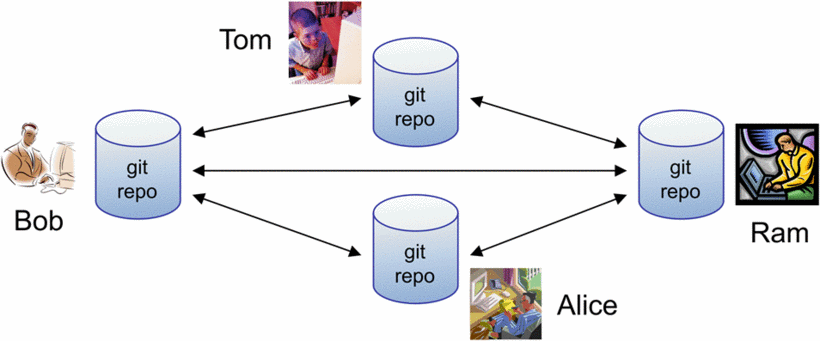
\includegraphics[width=1.0\textwidth]{decentralised_git.png}
\caption[Distributed revision-control with Git]{Distributed revision-control with Git. Figure taken from \cite{TorvaldsGit}.}
\label{decentralised_git}
\end{figure} This section will first provide a quick introduction into Git \cite{TorvaldsGit}, then it will describe Git's pitfalls when used for code-mining, and finally it will explain how these pitfalls are tackled when Git is used for \fxch{}.
\subsection{Overview}
The main difference between Git and other VCSs, say Subversion (SVN), is that Git is fully distributed: each developer's machine has a valid Git repository to which the developer can commit to, without accessing any `main' repository. Later the developer can push changes from the local repository to any other machine which they have access to, as seen in the figure \ref{decentralised_git}.

Despite this, usually there is a dedicated `origin' computer which holds the up to date version of a repository, and with which the developers are communicating. This approach makes it easier to develop software when internet connectivity is poor (as we can still work on a project locally), but introduces other issues, such as merge-conflicts (more on this later). 

Since its development in 2005, Git has been widely adopted by variety open-source projects as their primary VCS, such as the Django Project\footnote{https://www.djangoproject.com/}, Ruby on Rails\footnote{http://rubyonrails.org/} or jQuery\footnote{https://jquery.com/}.
\subsection{Git snapshots}

Git stores data differently to other major VCSs. Rather than storing for each file the list of changes, git stores the whole repository at each  point in the history. For efficiency if a file hasn't been changed at a commit, rather then storing the file again, Git only stores a pointer to the last identical file in the previous revision as in figure \ref{snapshot_git}.

We can think of a Git repository as an ordered list of snapshots. As follows, version-control is simply done by creating snapshots (by committing) of our repository. To view differences (using the \texttt{git diff} command) Git simply looks up the difference between snapshots
\begin{figure}[h]
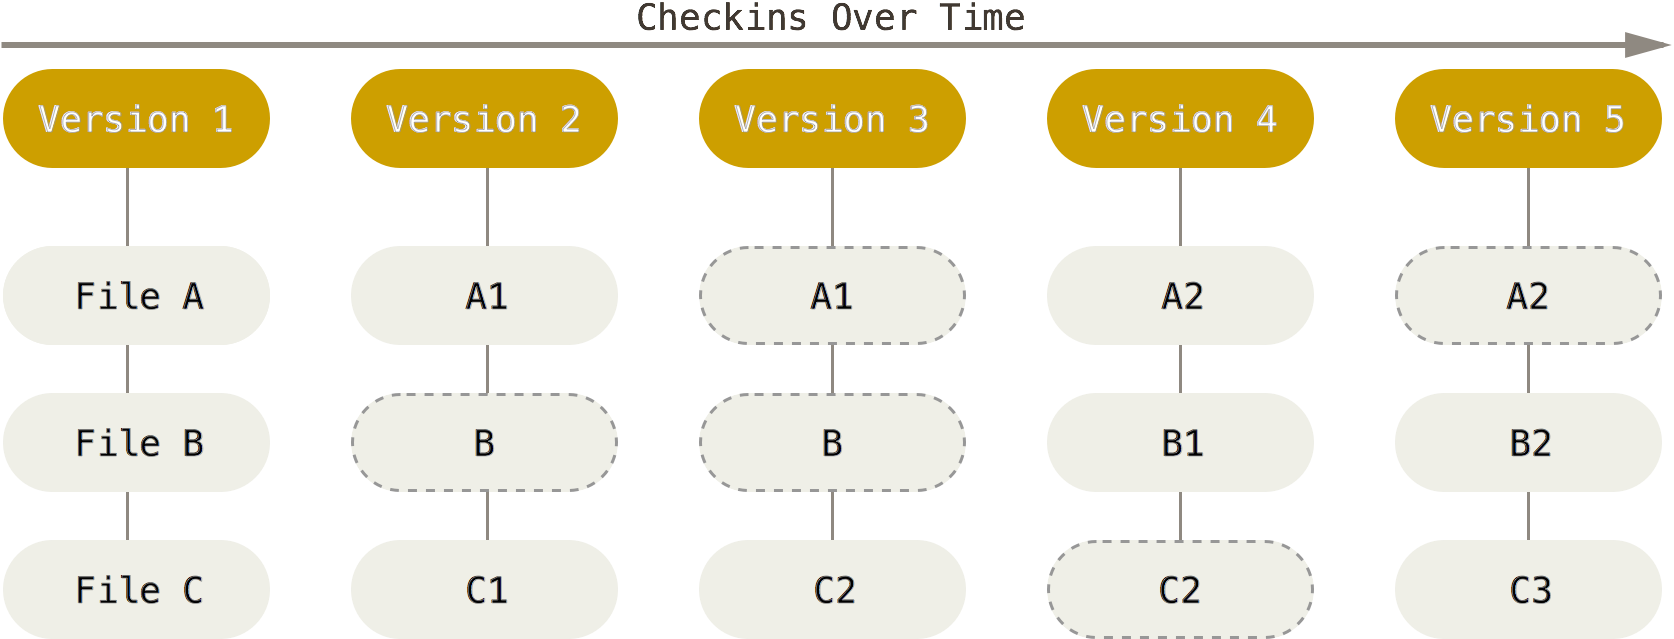
\includegraphics[width=0.8\textwidth]{snapshots_git.png}
\centering
\captionsetup{width=0.8\textwidth}

\caption[Snapshots in Git]{Snapshots in Git, pointers to files have striped lines. Figure taken from https://git-scm.com/book/}
\label{snapshot_git}
\end{figure}
\subsection{Git File structure}
In Git, we can think of a repository as a small file structure (one for each snapshot). Objects in this file structure can either be \textit{blobs} or \textit{trees}: blobs correspond to files whereas trees correspond to directories and sub-directories under the repository's root directory. At each point in the history of a repository Git stores a commit object, which stores the meta-data (time committed, author) about that commit.

Each commit object has pointer to a tree object, corresponding to the root directory of the repository at a given snapshot, as seen in figure \ref{commit-and-tree_git}. Each tree can have a pointer to many more trees or blobs, whereas blobs are leaf nodes. Each commit has a pointer to it's parent(s), except the special initial commit which does not have parents.
\begin{figure}[h]
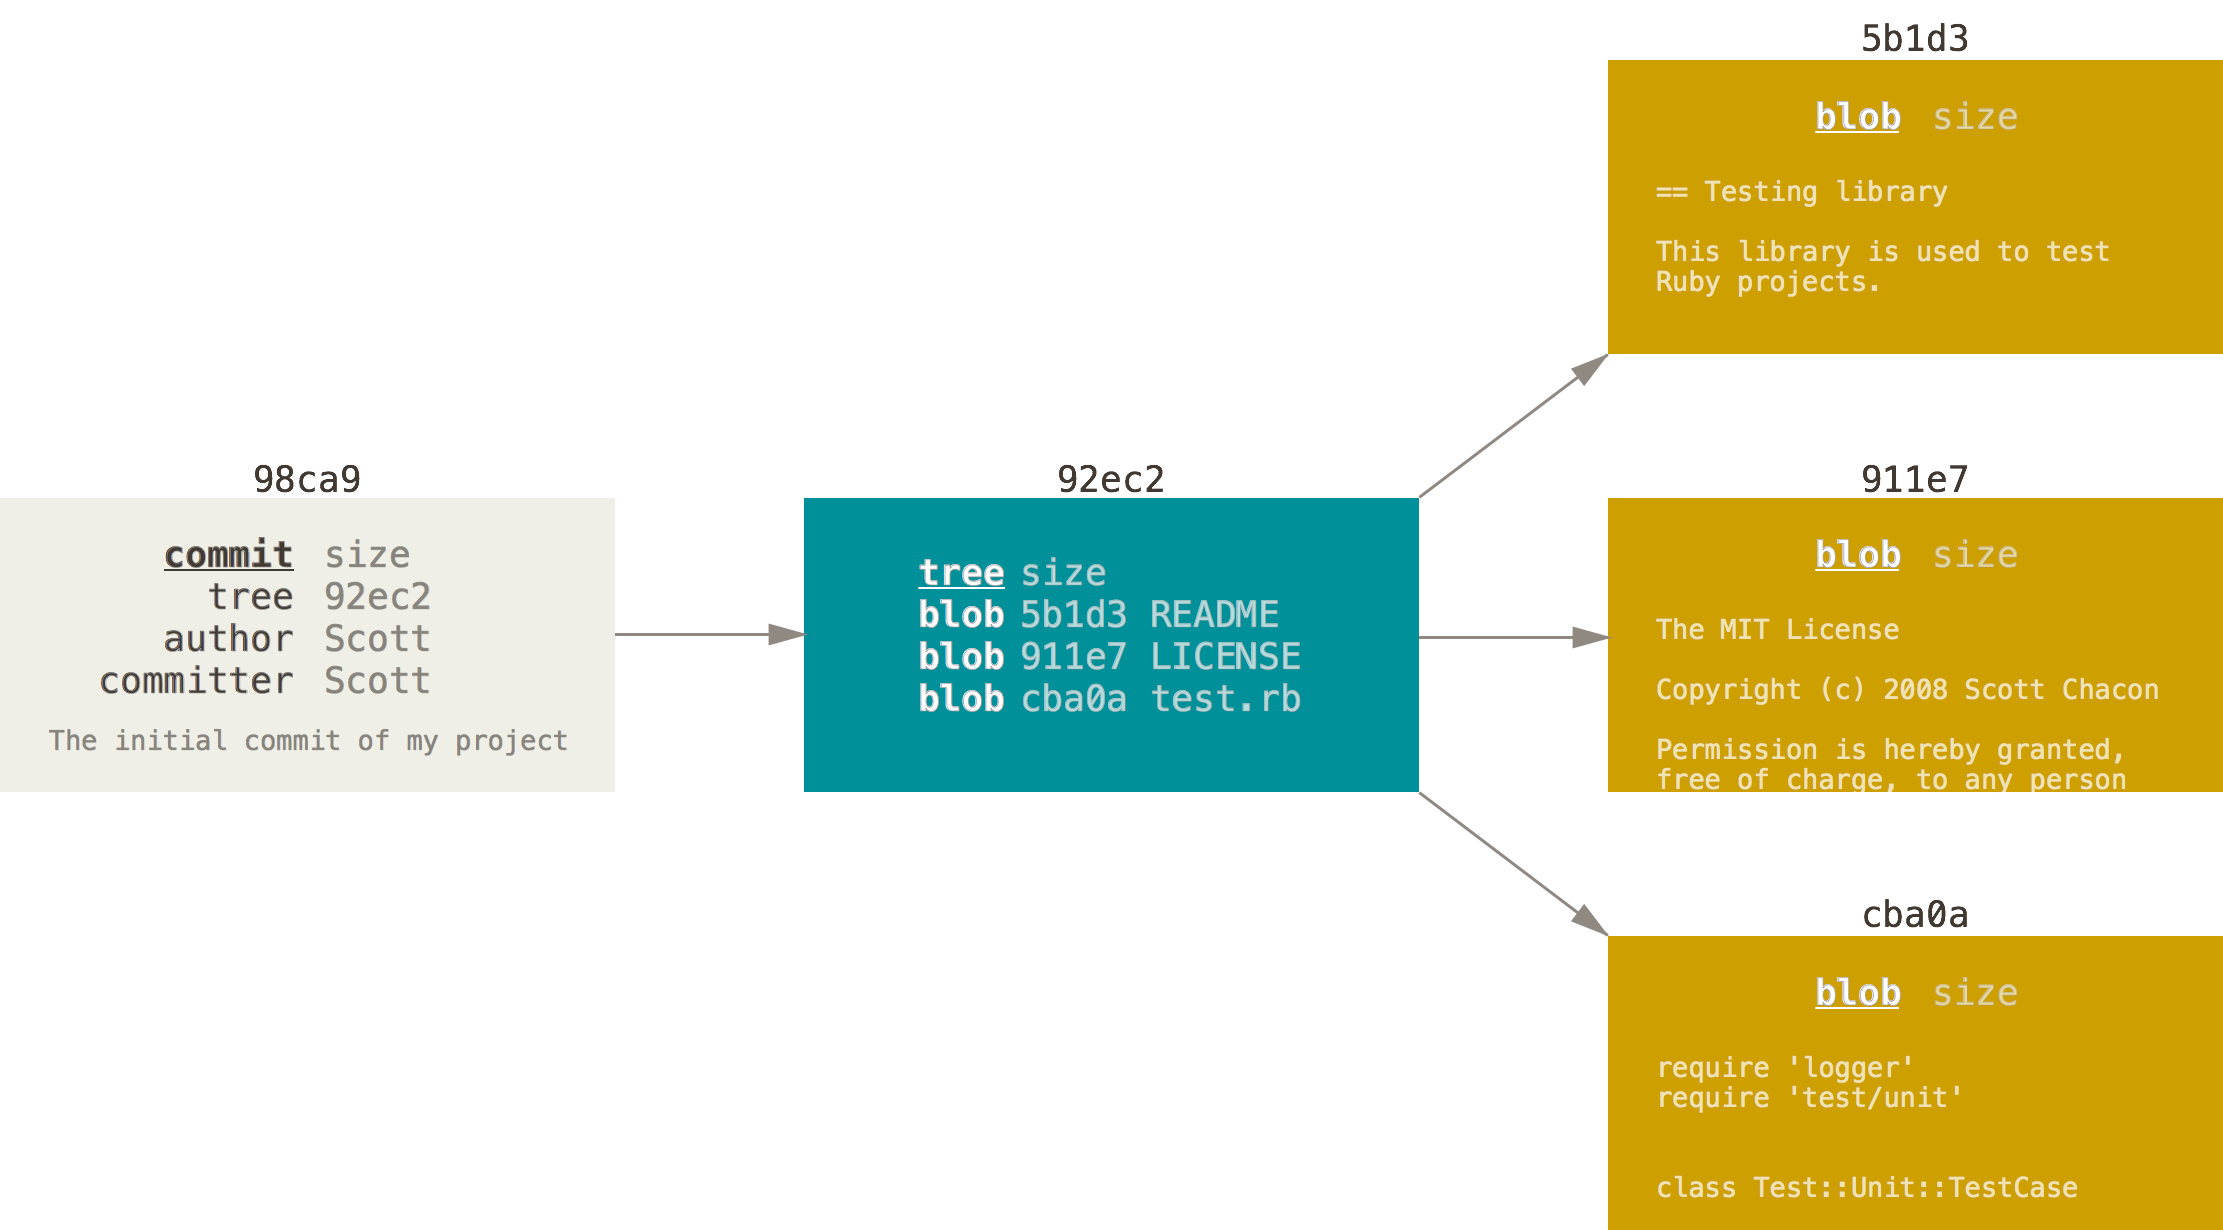
\includegraphics[width=0.8\textwidth]{commit-and-tree_git.png}
\centering
\captionsetup{width=0.8\textwidth}
\caption[Git file-structure for a given commit.]{Git file-structure for a given commit. Figure taken from https://git-scm.com/book/.}
\label{commit-and-tree_git}

\end{figure}
\subsection{Branches in Git}\label{gitbranches}
Branches are an important feature of Git, but they make mining repositories harder, as they introduce new problems to be tackled. They allow non-linear development in a decentralised manner, meaning that developments can make their own changes locally, and later join/merge these changes together. 

As discussed before each commit is simply an object with some meta-data, which stores a pointer to a snapshot. A branch is simply a pointer to one of these commits.

The branch named `master' is the default branch (although this can be changed); after initialising a repository you are given a `master' branch which will store a pointer to the latest commit made. When a new branch is created, Git creates a new pointer to the commit viewed at that moment. Git knows which branch is active at any time by storing a special pointer called `HEAD' which is a pointer to the active branch.
\begin{figure}[ht!]
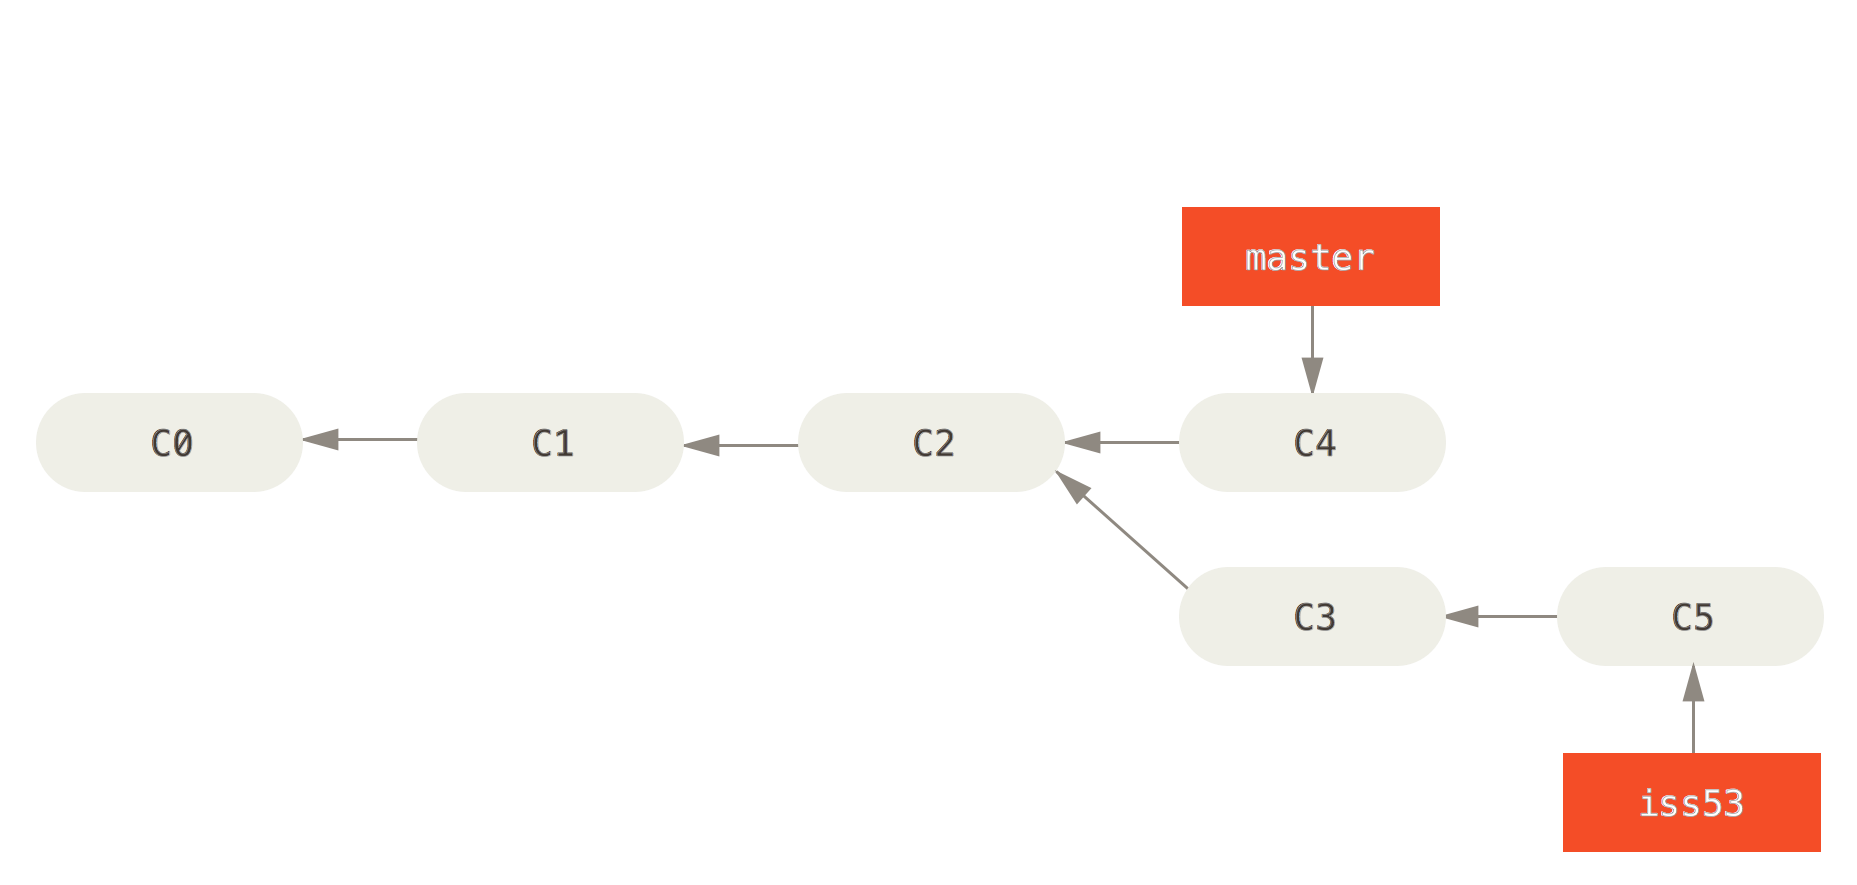
\includegraphics[width=0.8\textwidth]{basic-branching_git.png}
\centering

\captionsetup{width=0.8\textwidth}
\caption[Basic branching in Git]{Basic branching in git, with two branches: `master' and `iss53'. Figure taken from https://git-scm.com/book/.}
\label{basic-branching_git}
\end{figure}

\subsubsection*{Diverging branches}
It is possible to diverge two branches, as seen in figure \ref{basic-branching_git} above. There starting from commit C2, some changes were made on branch `master' which resulted in commit C4. Then, from C2 also some changes were made on branch `iss53', which resulted in branches C3 and C5. We can see from the diagram that C4 and C3 have the same parent, C2.

\subsubsection*{Merging branches}
Following this logic, you can also merge two branches, that is for example include the changes (that is the set of commits) made on branch `iss53' to the changes made on `master'. If the two branches are on the same linear path, we can simply `fast-forward', that is point the pointer of `master' to the same place when `iss53' is pointing. Otherwise, we need a real merge, which can be tricky to do automatically.

Figure \ref{basic-merging_git} shows how merging works in Git. We are merging `iss53' into `master', so the commit C5 has to appear on the `master' path as well.
\begin{figure}[ht!]
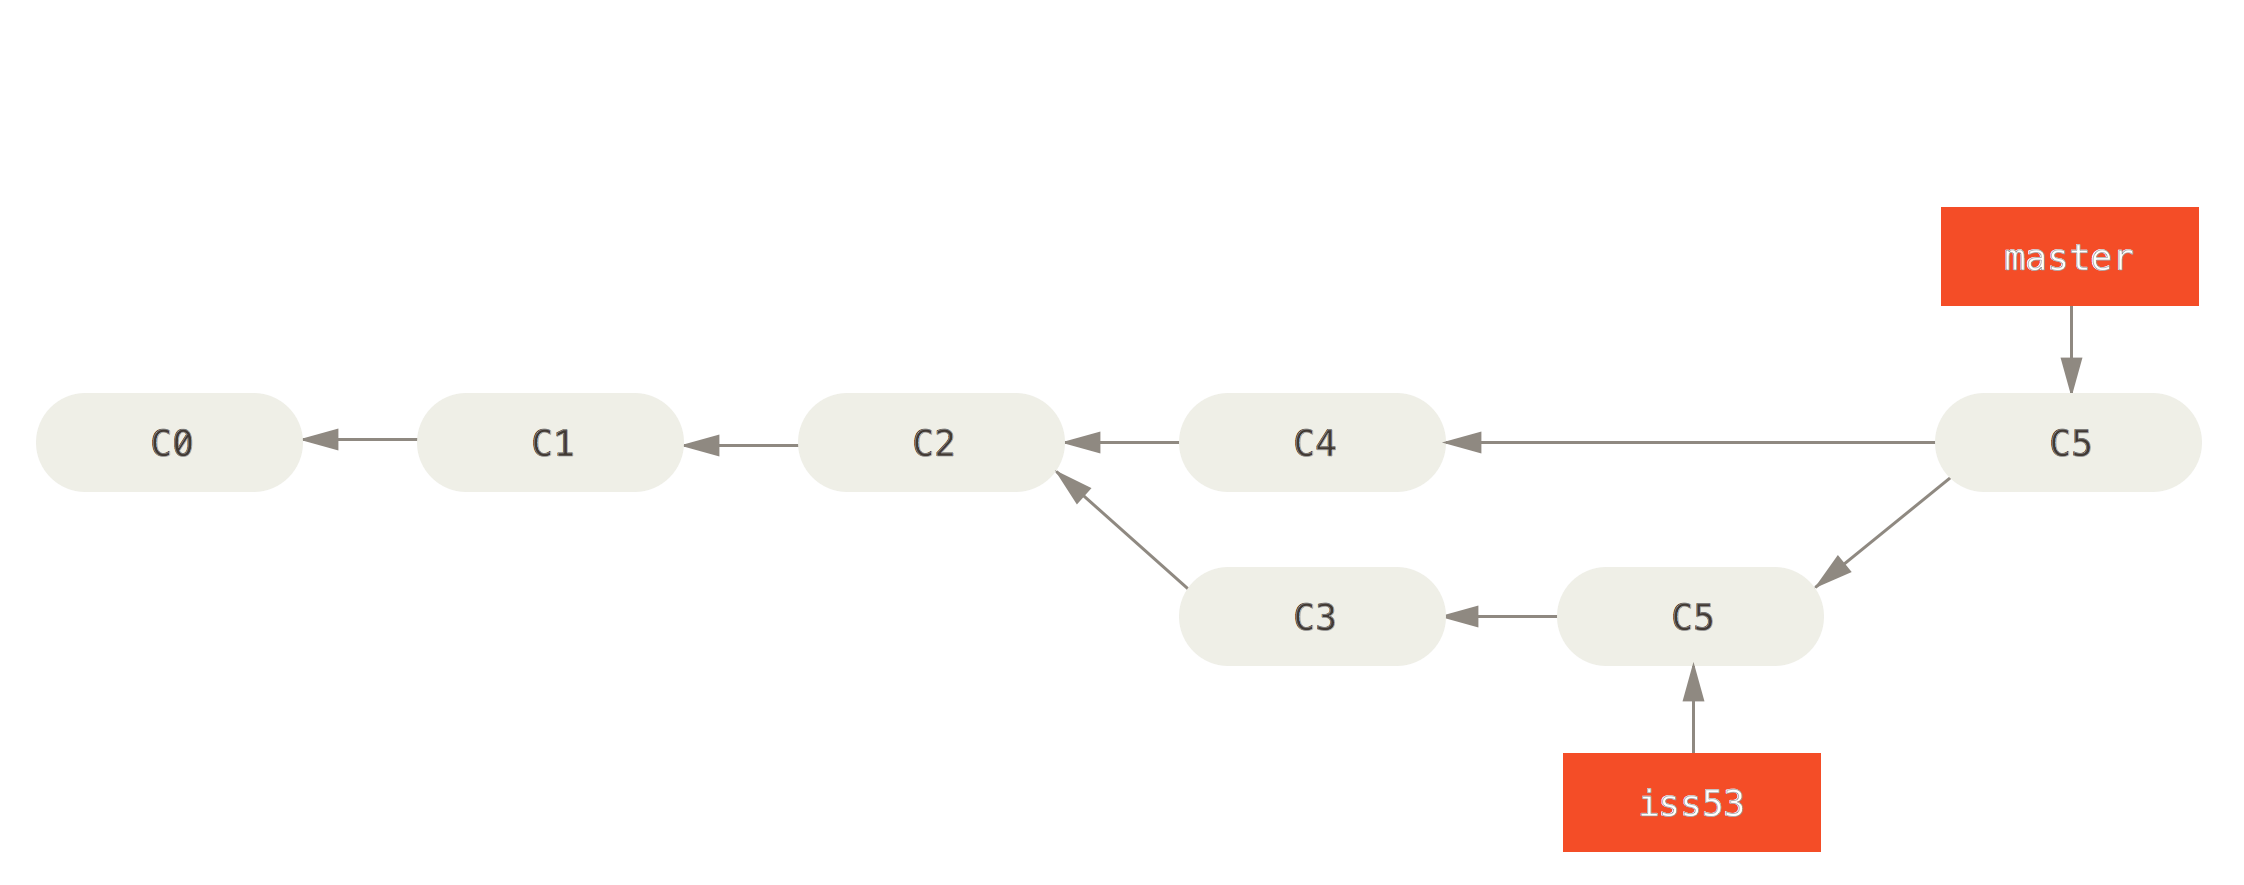
\includegraphics[width=0.8\textwidth]{basic-merging_git.png}
\centering

\captionsetup{width=0.8\textwidth}
\caption[Merging branches in Git]{Merging `iss53' branch into the `master' branch. Figure taken from https://git-scm.com/book/.}
\label{basic-merging_git}
\end{figure}

When performing a merge, there are two possibilities:
\begin{enumerate}
\item There are no merge-conflicts. This means that there is no single file which were changed/overwritten on both branches. In this case Git will handle merging automatically through a so-called ``recursive-merging'' by default.
\item There are merge-conflicts. This means that there is at least file which has been modified by both branches `master' and `iss53'. In this case Git will merge the files that it is able to merge, and for those where the conflict arose it will place some readable text to tell the user where the conflict is. The user will have to manually go to each file and resolve the conflict, and commit the new changes later. There exist automated tools for merge-conflict resolution, which automate the last two steps during the merging command itself.
\end{enumerate}

When a merge occurs Git will create an automated merge commit, as seen in figure \ref{basic-merging_git}. If there are no merge-conflicts (as seen above) a new merge-commit is created (copy of C5) which will contain the same changes which were made at C5, but it will have two parents: C5 on `iss53' and C4 on `master'. In this case, changes made by C5 will appear twice: once on branch `iss53' and once on branch `master'.

If there are merge-conflicts, our new merge-commit will contain the changes which resolved that conflict, so C5 will only appear once on branch `iss53'.

A key difference between Git and other VCS is that in Git we can treat the repository as a Directed Acyclic Graph (DAG) of commits, as the branching data is preserved, as we can see in figure \ref{branching}
\begin{figure}[h]
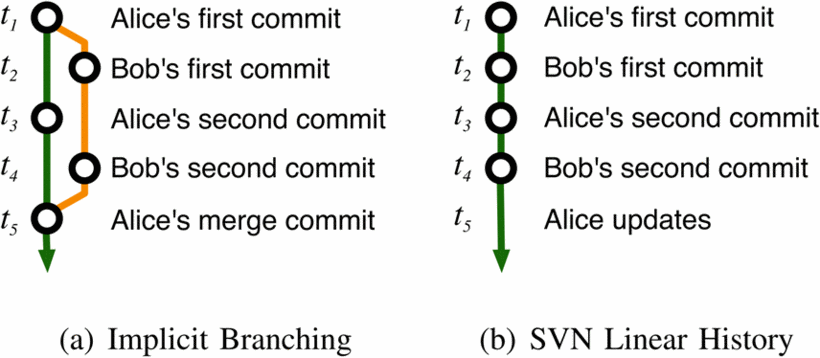
\includegraphics[width=0.8\textwidth]{branching.png}
\centering

\captionsetup{width=0.8\textwidth}
\caption[Comparing Git branching with other VCS]{Comparing Git branching with other VCS. (a) is the DAG produced by git, while (b) is the linear history produced by SVN. Figure taken from \cite{Git}}
\label{branching}
\end{figure}

Alice's merge commit will have two parents: Alice's second commit and Bob's second commit, thus preserving the DAG information, which is lost in SVN. This DAG representation comes handy when analysing how exactly each user contributed to a repository, but it makes backtracking a commit history more complex, as we might want to go through all the paths in the DAG. This will increase the complexity of some code-mining and repository-mining algorithms \cite{Git}.


\subsubsection{Using Git for \fxch{}}
Luckily, it is also possible to view the commit history as a linear list of commits (even when with merges present). We simply take each commit in the DAG and order them by their committed time, regardless on which branch were they made.

However, this linear representation might contain duplicates in Git (for the merges without merge-conflicts), as seen in figure \ref{basic-branching_git}:  C5 will appear twice in our linear representation, once as a merging commit and once as a part of `iss53'. We will use this linear representation when implementing \fxch{}.
\section{GitPython}

\subsection{Overview}
GitPython\footnote{https://github.com/gitpython-developers/GitPython} is a Python package developed by Sebastian Thiel\footnote{https://github.com/Byron} as a pure Python high-level tool for interacting with Git repositories. It provides a mechanism for reading and writing Git objects by using Python code. Also it allows us to use Git functionality (creating new repositories, committing changes, checking-out branches etc.) through function calls in Python.

When implementing \fxch{}, GitPython will only be used to access for the following tasks:
\begin{itemize}
\item Getting the list of commits (for the \texttt{master} branch) in chronological order, by their committed time.
\item Determining differences in files between two commits.
\item Keeping track of each file's history: number of changes, faults and lines at each commit.
\end{itemize}
\subsection{The object database}\label{dbbackend}

\begin{figure}[h]
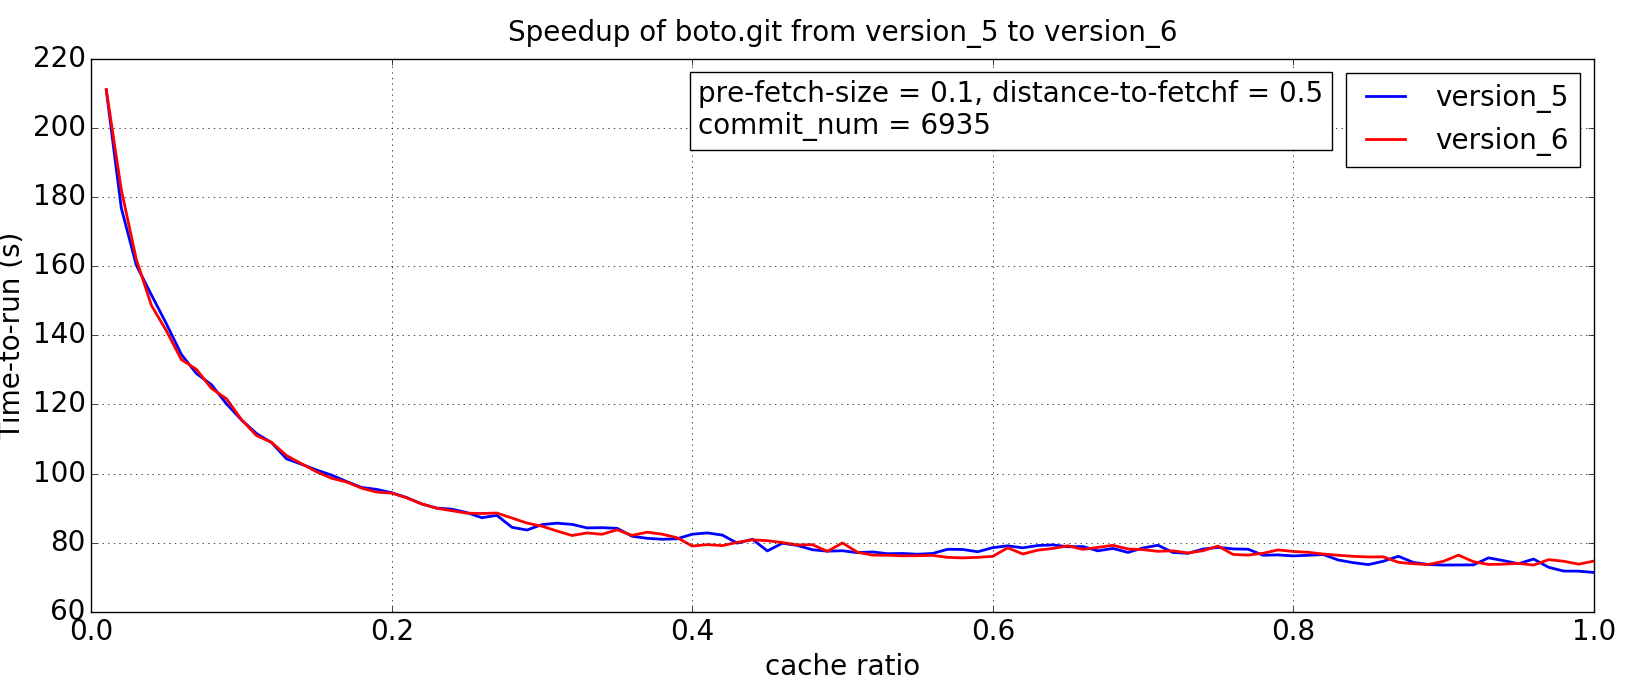
\includegraphics[width=1.0\textwidth]{db_backend-1.png}
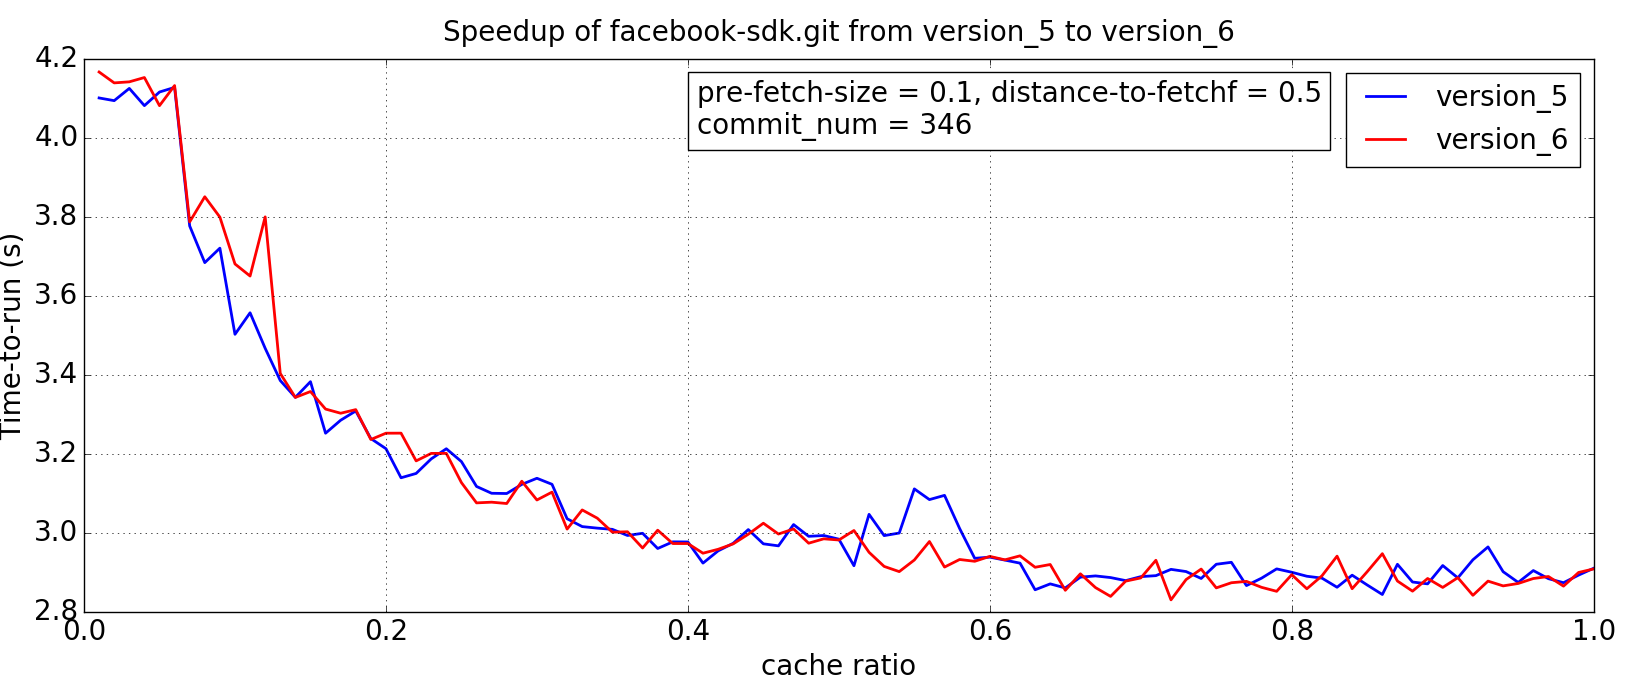
\includegraphics[width=1.0\textwidth]{db_backend-2.png}

\captionsetup{width=0.95\textwidth}
\caption{Showing time-to-run of back-ends \texttt{GitDB} (version\_5) and \texttt{GitCmdObjectDB} (version\_6) for repositories boto.git and facebook-sdk.git when \fxch{} is run for different cache-ratios. Here cache-size is computed directly from the cache-ratio, which will be explained in Chapter 3 in detail.}
\label{boto_gitdb}
\end{figure}
Behind the scenes GitPython is using a Git object database when accessing a Git repository. We have two options provided by GitPython: either we use the default \texttt{GitDB} (first implemented in the package gitdb\footnote{https://pypi.python.org/pypi/gitdb}, then added to GitPython) or we use \texttt{GitCmdObjectDB}. The first one, according to the Thiel \textit{"uses less memory when handling huge files, but will be 2 to 5 times slower when extracting large quantities
small of objects from densely packed repositories"} while second one \textit{"uses persistent git-cat-file instances to read repository information. These operate very fast under all conditions, but will consume additional memory for the process itself. When extracting large files, memory
usage will be much higher than the one of the \texttt{GitDB}"}.


Figure \ref{boto_gitdb} shows the time-to-run in seconds for both. As it can be seen, there is not a significant difference in the running time, so the default (\texttt{GitDB}) back-end was used for all further analyses.

The reason why it is more efficient to use gitdb is due to how gitdb handles memory usage. Rather than loading all the Git objects to the memory, it will operate on streams of data, which will ensure that our object database can handle objects of any size.
\cleardoublepage
\chapter{Implementation}
This chapter explained the main components implemented to run \fxch{}. It first explores a very high level view of all modules, and then it describes all components in more detail, together with any implementation difficulties. Finally, this chapter will talk about the bottleneck of the first implementation, and how this bottleneck was tackled to achieve a speed-up.
\section{Design overview}

The algorithm is implemented in Python using its 2.7.6 release. The implementation has several modules which handle different parts of the algorithm, the main module being the Repository module which implements the algorithm itself. We use several other back-end modules, such as Parsing, File-management and Cache. Figure \ref{fixcache_flowgraph} on the next page shows these main modules and how do these modules depend on each other.

\begin{figure}[h]
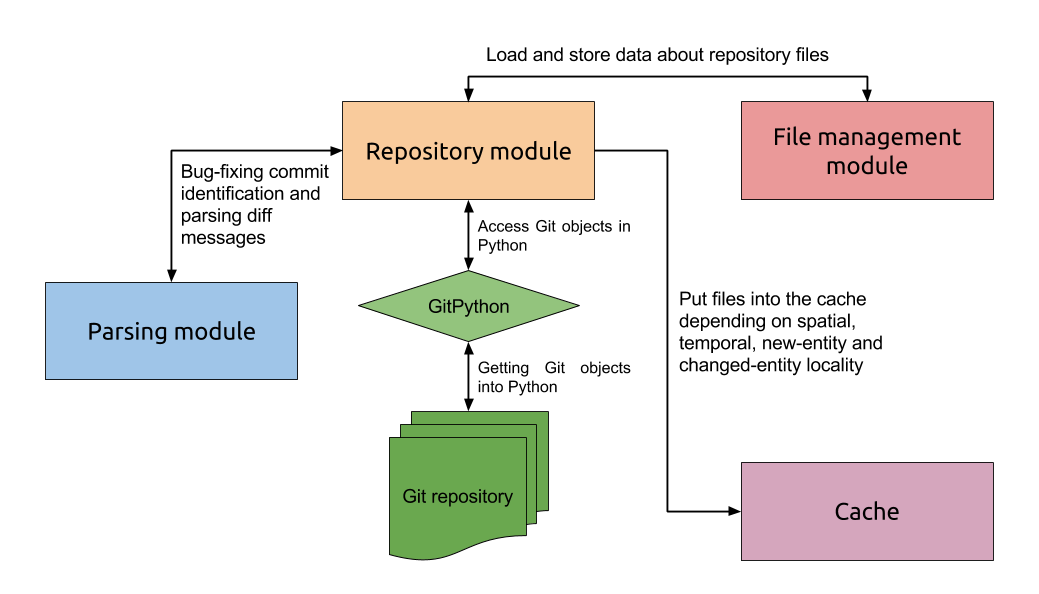
\includegraphics[width=1.0\textwidth]{fixcache_flowgraph.png}

\captionsetup{width=0.9\textwidth}
\caption[Core modules and the interaction between them.]{Core modules and the interaction between them. Lines indicate in which direction the data flows between modules.}
\label{fixcache_flowgraph}
\end{figure} 

\paragraph{Parsing module}Accepts data from Repository (as can be seen in figure \ref{fixcache_flowgraph}), and then it processes that data and sends the parsing result back to the Repository. It is essentially a collection of functions implementing different parsing functionalities used by \fxch{}: flagging important lines, parsing \texttt{git diff} messages to get the line numbers of deleted lines and flagging bug-fixing commits from the commit message.

\paragraph{File-management module}Implements a layer for representing files, file-sets and distances between files. The classes implemented by this module are used both by the Cache module and by the Repository module, however only the latter accesses File-management explicitly. We can think of this module as a database which can be queried by the Repository module for different types of data such as file-metrics and relationships between files.

\paragraph{Cache module}This module contains the \texttt{Cache} class which implements the cache functionality used by \fxch{}. Repository will look-up files in the Cache module and it will send new files to our Cache module. Cache will handle these additions: it will add the arriving files, and it will remove files if the cache is filled to make space for arrivals. Removing is handled implicitly by our module, hence the one-way line figure \ref{fixcache_flowgraph}.

\paragraph{Repository module}This is the main module which runs \fxch{} itself. It will communicate with all the other modules, also it will monitor the communication of these module between themselves. Moreover, this module will be in charge of accessing the Git repositories, through GitPython.
\section{Back-end modules} Back-end modules are used by the Repository module, when running \fxch{}. They are the layer which handles the abstraction of objects and object metrics used by \fxch{}.

\subsection{Parsing module}\label{parsing}
The Parsing module parses data arriving from the Repository module, as it can be see in the figure \ref{parsing_module} representing the data-flow through the module. The three key functionalities implemented are: deciding whether a line is ``important'' or not; getting the numbers of deleted lines from the output of a \texttt{git diff} command; parsing the commit messages to identify fixing commits. 
\begin{figure}[h]
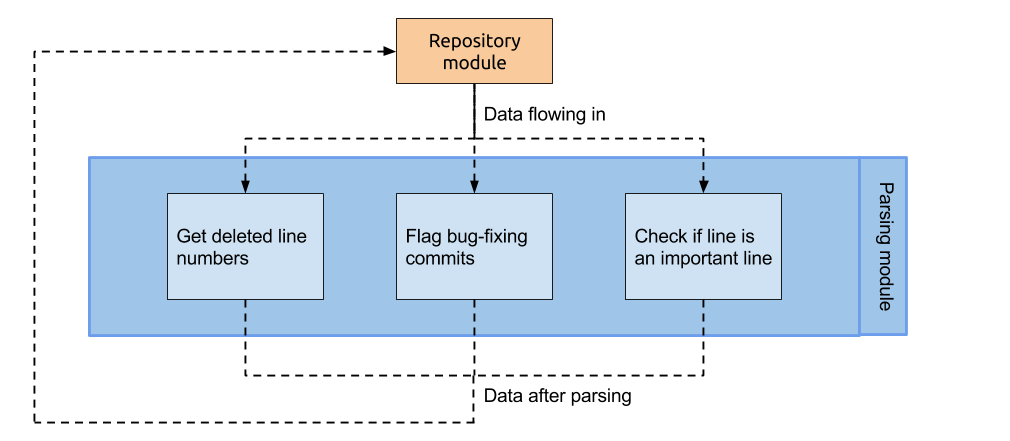
\includegraphics[width=1.0\textwidth]{parsing_module.png}
\caption{Data-flow through the Parsing module}

\label{parsing_module}
\end{figure}
\subsubsection*{Check if line is important}
When identifying bug-introducing commits, we are using the SZZ algorithm (explained in section \ref{szz}), which has a step of finding which lines are contributing to the bug. The algorithm assumes that each deleted line between a fixing commit $C_{fix}$ and it's parent contributed to the bug fixed by $C_{fix}$.
\clearpage
This assumption has been criticised by Kim \etal{} \cite{KimZim} as it treats all lines equally important, which might ultimately introduce plenty of false-positive lines, that is lines which were deleted between $C_{fix}$ and it's parent, but had no contribution to the fixed bug whatsoever.
\begin{figure}[t]
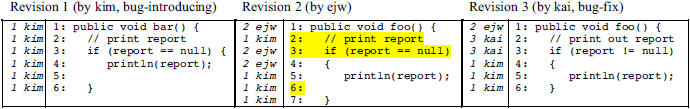
\includegraphics[width=1.0\textwidth]{automatic_identification.jpg}
\caption[Example of changes between revisions.]{Example of changes between revisions (3rd fix is a bug-fix change). Figure taken from \cite{KimZim}.}
\label{automatic_identification}
\end{figure}

Figure \ref{automatic_identification} provides an example. Looking at the bug-fixing revision (Revision 3) we can see that it changed lines \#2 and \#3 (that is removed \#2 and \#3 and inserted new lines to that position) and it removed line \#6.
SZZ would identify all of these lines as buggy lines, whereas we can see that truly only \#3 should be treated as a buggy line, because \#2 is a comment line and \#6 is blank line.

Several improvements have been proposed by Kim \etal{} to reduce the number of false-positives, out of these we are only checking if a line is blank/empty or if it is a comment line \cite{KimZim}. As this implementation is for Python repositories, to identify comment lines we parse each line and identify whether it starts with \texttt{\#} (the comment symbol in python). Multi-line comments are ignored, as python uses the same syntax for them and for mutli-line strings. 

This important line checker merely outputs an approximation for the lines which are truly important (that is they contributed to the bug fixed), usually it will return a bigger set. Further approximation of the true set would require more techniques mentioned by Kim \etal{}, but getting the exact set is computationally impossible \cite{KimZim}. 
\subsubsection*{Getting deleted line numbers}
An essential part of the \fxch{} algorithm is identifying which lines were removed between two revisions. This information is later used by SZZ algorithm when identifying bug-introducing commits.

Our module will accept the output of a \texttt{git diff} command for each file in the commit, and it will pars this output to get the line numbers which were deleted in that \texttt{git diff} (where the difference is what changed between a commit and it's parent commit), that is the line numbers of all the lines starting with ``\texttt{-}'' in our \texttt{git diff}.
\subsubsection*{Identifying bug-fixing commits}
For each commit the algorithm looks at, we need to decide whether it is a fixing-commit or not. To identify these commits, we need to parse the commit message itself. If the commit message is accepted by any of the below regular expressions (following Sadowski \etal{} \cite{Sadowski}), we flag it as a bug-fixing commit. 

Regular expressions used to flag bug-fixing commits:
\begin{itemize}
\item \texttt{r'defect(s)?'}
\item \texttt{r'patch(ing|es|ed)?'}
\item \texttt{r'bug(s|fix(es)?)?'}
\item \texttt{r'(re)?fix(es|ed|ing|age\textbackslash s?up(s)?)?'}
\item \texttt{r'debug(ged)?'}
\item \texttt{r'\textbackslash\#\textbackslash d+'}
\item \texttt{r'back\textbackslash s?out'}
\item \texttt{r'revert(ing|ed)?'}
\end{itemize}
\subsection{File-management module}
When running \fxch{}{} we need to somehow store data about the files we looked at so far (data to store: number of faults, changes, their LOC) and also we need to store the distance between any two files in our system, at any commit. A  good implementation would be able to tell for any two files $f_1$ and $f_2$ what is their co-occurrence (which is inversely proportional to their distance) at any commit $n$. Figure \ref{filemanagement_module} shows a high level view of the File management module, and how does data flow through it.
\begin{figure}[h]
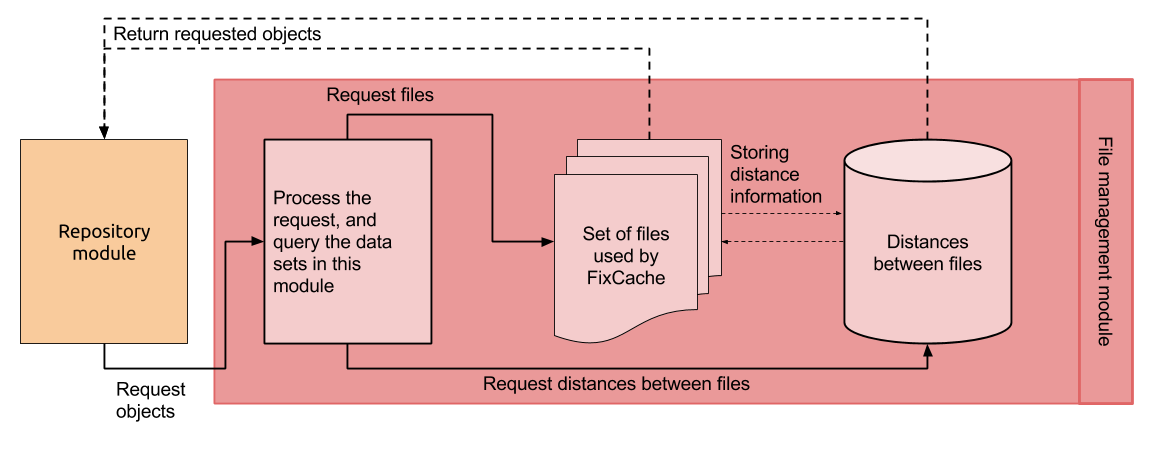
\includegraphics[width=1.0\textwidth]{filemanagement_module.png}
\caption{Data-flow through the File-management module}
\label{filemanagement_module}
\end{figure}

As it can be seen from the figure, Repository requests objects (\texttt{filemanagement.File} or \texttt{filemanagement.Distance} objects) from the File-management module, and the module will return the requested objects from a set of files or from the distance database.
\subsubsection*{Processing requests}
When requesting files, the Repository module accesses them only by their file-path. That is, it queries every \texttt{filemanagement.File} object by it's file-path, and the File-management module will either return the corresponding file, or if it did not exist before, it will create a new file with the queried path, and return this newly created file. We can think of this as a dictionary functionality with an extension that if a key looked-up is missed, this module will create the corresponding value, rather than throwing a \texttt{KeyError}.

Similarly for file-distances, Repository will query File-management by file-path, only this time the request will contain two paths (of the files we want to know the distance of). From these two paths, the Distance-database will create a key, and as before, it will return the corresponding value, or create a new \texttt{filemanagement.Distance} object. The key-generation is fairly simple:
\begin{gather*}\label{distance_key} 
	\forall f_1, f_2\ files \\
	key(f_1, f_2) = \begin{cases}
						f_1.path+f_2.path &if\ f_1.path > f_2.path\\
						f_2.path+f_1.path &if\ f_1.path < f_2.path\\
						error &otherwise: two\ paths\ equal, f_1 == f_2
					\end{cases}
\end{gather*}
That is we will append the shortest path to the longest path for any two files. If the two paths are equal, it means that the two files looked at  are also equal, and we need to throw an error. Generally, this will never happen in this \fxch{} implementation, as we never query the distance with the same path.
\subsubsection*{Storing file information}
For each file in the repository looked at when running \fxch{} we create a \texttt{filemanagement.File} object indexed by it's path, which will store the basic information needed by \fxch{} as mentioned above. Whenever an file-related event occurs during a \fxch{} run we need to change or update the internal data of the files involved in the event so that they have a correct state when used by \fxch{}. There are three three major file-events:
\begin{itemize}
\item \textit{Changed file}: whenever a file is committed, we need to record this change at that commit. First we add the commit number to the changed-commit-list (which stores all the commits at which the file was changed). Then we need to update the LOC for that file, where the amount of lines changed will be equal to $added\_lines - deleted\_lines$.
\item \textit{Fixed fault}: at each bug-fixing commit $C_{fix}$, for each file involved, we mark that there was a fault associated with that file, and that this was fixed at $C_{fix}$. This is later not used, as we are using LRU cache-replacement policy, but it could have been used with different cache-replacement policies which take the number of faults and their occurrence in time into account.
\item \textit{Reset the file}: To complete an analysis we need to run \fxch{} 1500 times (for the cache-ratio analysis). If our repository, say has a 1000 files, we would create 1.5 million \texttt{filemanagement.File} instances (not taking into account any garbage-collector). This would be rather inefficient, so instead we reset all the objects present in our File-set and Distance-database: we set their internal parameters to their initial values.
\end{itemize}

Rather than requesting each file individually at these events, the output of a \texttt{git diff -{}-stat} command is passed as data to the File-management module, which will update and return files accordingly. In Git, this output looks like this:
\vspace{0.2in}
\begin{lstlisting}[language=bash, tabsize=4, backgroundcolor=\color{lightgray}, keywordstyle=\color{black}, frame=single, framesep=10pt, xleftmargin=10pt, xrightmargin=10pt]
setup.py | 11 ++++++++++-
 1 file changed, 10 insertions(+), 1 deletion(-)
\end{lstlisting}

\clearpage
Luckily we do not need to parse this, as GitPython already has a parser, which will parse it and create a nested Python dictionary from the parsed data. For the output above, this dictionary will look like this:

\begin{lstlisting}[language=Python, tabsize=4, backgroundcolor=\color{lightgray}, keywordstyle=\color{black}, frame=single, framesep=10pt, xleftmargin=10pt, xrightmargin=10pt]
{ 
	u'setup.py': {
    	'deletions': 1,
	 	'lines': 11,
	 	'insertions': 10
	}
}
\end{lstlisting}

Each changed file's path will be a key in this dictionary, and the corresponding value will be an another dictionary with three keys: \texttt{deletions, lines, insertions}. Our module will use this parsed \texttt{diff} data to update and create new files in our File-management module. Furthermore, File-management will clean-up deleted files, based in this data: we assume that each file is deleted when their LOC becomes zero.

Once File-management finished updates and deletes, it will return the \texttt{filemanagement.File} instances for all the files involved in this update.
\subsubsection*{Distance-database}
In order to implement the temporal locality used by \fxch{}, we need to know the co-occurrence of any two files at any commit. To store that, for each two files committed together a \texttt{filemanagement.Distance} instance will be created and stored in the Distance-database. This instance will have a list of commit numbers representing the commits when the two files were changed together. That is, for each two files in a commit, we either update the corresponding \texttt{filemanagement.Distance} object, or we create a new one if it has not yet existed.

Whenever two files are committed together (say at commit $C_n$, the Repository module will query the Distance-database (using the key generated as explained in \ref{distance_key}) to get the \texttt{filemanagement.Distance} object, and it will update the co-occurrence for that object, that is add $C_n$ to the commit list.

The Distance-database is also important when determining which files are the closest ones to a given file $f$ at a given commit $C_n$. In this case, the Repository queries the Distance-database with one file path ($f.path$ in this case), and asking for $k$ closest, files, and the database will respond with a list of $k$ \texttt{filemanagement.File} objects with the highest co-occurrence with $f$ (that is lowest distance to $f$).
\subsection{Cache implementation}
\fxch{} uses the notion of a file cache, which has some limited number of files in it. We can think of it as a bucket, where we can put some files in, and when the bucked is filled, it will automatically remove some files in order to make space for new arrivals. The \texttt{cache.Cache} class is responsible for keeping track of files which are in the cache, it also counts cache-hits  and cache-misses, and as mentioned before, it will remove files when the cache is filled (according to the LRU policy). The figure \ref{cache_module} shows the cache handles the addition of new files.

\paragraph{Pre-processing}
Before putting the files into the cache, there is a pre-processing step, which will check if either of the files is already in our cache. If so, we will simply discard those files to avoid duplicates. This step is important as our cache needs to know exactly how much free space is required upon new arrivals.

The pre-processing step may also include sorting, if the cache is smaller than the number of files we want to insert. In this case, we need to sort them so that later they obey the LRU cache-replacement policy.
\begin{figure}[h]
\centering
    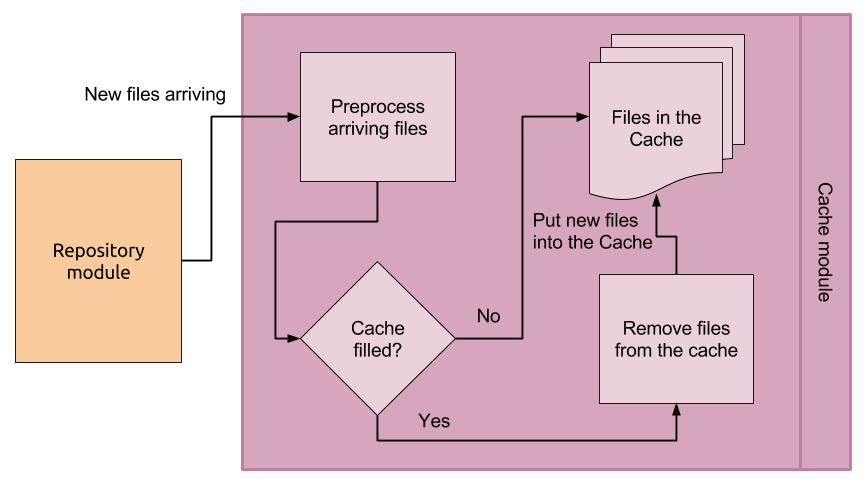
\includegraphics[width=0.75\textwidth]{cache_module.png}
  \caption{Adding new files to the Cache and processing them.}
  \label{cache_module}
\end{figure}

\paragraph{Adding new files} After pre-processing we can add the arriving files to our cache. We first look-up how much space do we need, and remove files accordingly. Once the required space has been freed, we can safely add the new arrivals.

\paragraph{Removing files} We are not removing any files explicitly. The implementation itself will take care of clean-up, so that it will only discard files when our cache needs more space. As we are using the LRU cache-replacement policy, if we need a space of $k$ files, this module will select the top $k$ least recently used (changed/committed) files and remove them from the cache.

\paragraph{Limiting the number of files}
Internally, files are stored in Python \texttt{set()} object, which does not allow duplicates, but it does not have a size limit by default. To actually have a limit in our cache implementation, all addition methods first look up how many files are currently in the cache, and subtract that value from the cache size to get how big is the currently available space. Removing files works accordingly to this: if we need more space, we remove as many files as necessary to free up the cache.
\clearpage
\section{The Repository module}
This module is the central element of \fxch{} implementation. It is connecting all modules together, and uses them to run and analyse the algorithm for different repositories. A \texttt{repository.Repository} class is instantiated for each Git repository we want to run \fxch{} on. Also, this module has two more classes, used only for evaluation purposes.
\subsection{Implementing the SZZ algorithm}
The SZZ algorithm in this implementation is implemented inside the \texttt{repository.Repository} class, rather than a standalone module, as it is a core part of \fxch{}.
The two functions which are implementing it are:
\begin{itemize}
\item \texttt{\_get\_diff\_deleted\_lines(self, commit1, commit2)}

Returns the deleted line-numbers (per file) between any two commits. Used to get the deleted lines between a commit and it's parent.
\item \texttt{\_get\_line\_introducing\_commits(self, line\_list, file\_path, commit)}

Once we have the line numbers which were deleted between two commits (commit and it's parent) we can for each file get the list of bug-introducing commits. This method uses the \texttt{git blame} (which, in GitPython outputs a nested list, where the first value of a list is a commit object, and the second value is a list of lines last changed - introduced - by that commit), and produces a list of bug-introducing commits.
\end{itemize}
The SZZ algorithm is used for identifying commits which introduced a bug, that is it is only called for bug-fixing commits.
\subsection{Cache size initialisation} A key variable used by our algorithm is the cache-size. Upon each initialisation we need to set the cache-size which will be stay static throughout a single run of the algorithm. To calculate the cache-size, we need to set a variable called cache-ratio (a number between between 0.0 and 1.0), and from this we will calculate the cache-size the following way: we take the number of files in the repository at the last commit, and we multiply this number by the cache-ratio. We then take the floor of this number (if the floor is zero, we add one, as the cache-size cannot be zero) to arrive at the desired cache-size. That is:
\begin{align*}
	cr = file\_count\_at\_last\_commit*cache\_ratio\\
	cache\_size = \begin{cases}
						1 & if\ floor(cr) = 0\\
						floor(cr) & otherwise
					\end{cases}\\
	where\ cache\_ratio \in (0.0\dots 1.0]
\end{align*}
To calculate the variable file-count-at-last-commit we need to traverse the Git tree at the last revision, and count the number of `blobs' (objects representing files) in the tree. 

\subsection{Setting variables} Once we calculated and set cache-size we can calculate other variables, such as distance-to-fetch (block-size) and pre-fetch-size as discussed in \ref{variables}. In the original paper all these variables are given as a percentage of file-count-at-last-commit, that is if file-count-at-last-commit = 100, then distance-to-fetch = 5\% means that we will fetch 5 files each time we use our spatial locality.

Rather than using percentages, this implementation for both distance-to-fetch and pre-fetch-size uses between 0.0 and 1.0. Also, they are not ratios of file-count-at-last-commit, but rather of cache-size. That is if file-count-at-last-commit is 100, cache-ratio is 0.1 and distance-to-fetch is 0.5, then the cache-size is 10 ($100*0.1$) and we will fetch $10*0.5 = 5$ number of files each time we use our spatial locality.

\subsection{Initialising commits} In Git each commit's identifier is a 40-digit long hexadecimal number generated by SHA-1 from the commit data, it is impossible to know just from the hash value what is the order of commits. Our \fxch{} is using integers as commit identifiers (the bigger the commit number, the later it happened), so a dictionary needs to initialised prior to running our algorithm. We first iterate through the list of commits (which is provided by GitPython) and at each commit we store the hash value of that commit as key, and it's order in the list as the value. Each time we want to access the order of any commit object, we can look-up this dictionary.
\clearpage
\subsection{Running \fxch{}}
\begin{wrapfigure}{r}{0.5\textwidth}
\begin{center}
\vspace{-16pt}
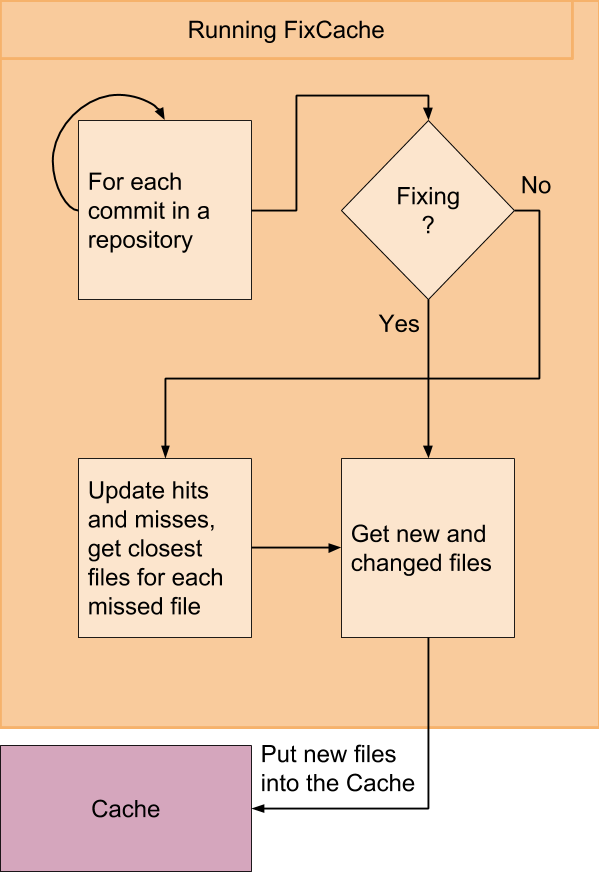
\includegraphics[width=0.5\textwidth]{repository_module.png}
\end{center}
\caption{Control-flow of \fxch{} inside the Repository module.}
\label{run_fxch}
\end{wrapfigure}
To run \fxch{} we need to call \texttt{run\_fixcache} on a \texttt{repository.Repository} instance; calling this method will run \fxch{} with the currently set parameters. However, before running the algorithm itself, we need to find the repository for which we want to run it on.

The Repository module will accept a string as an input, which will be the name of the repository we want to look at. The module will look for a repository with this name (under a pre-defined directory for repositories) and it will connect to it with GitPython, or throw an error if the repository is not found. Once we have connected to the desired repository we can run \fxch{}. The figure \ref{run_fxch} shows how the control-flow inside the Repository module works for a single run.

Between any two runs, we do not create a new connection with the repository, but rather we call a \texttt{reset()} function, which will implicitly reset the data found in the modules discussed so far. This reset propagation will save memory, and also save some time as it is not necessary to redo the initialization step before each run.

Once we have all these modules, implementing \fxch{} is quite straightforward. Following the figure \ref{run_fxch}, a more detailed pseudo code would look like the algorithm presented on the next page.
\clearpage
\begin{algorithm}[H]
\KwData{A Git repository; Initial settings}
\KwResult{A cache with files projected to have bugs in the future}
\For{each commit C in the commit list}{
	\uIf{C has no parents}{Pre-load the cache with some initial files, starting with ones with the highest LOC}
	\uElseIf{C has one parent}{
		\uIf{C is a bug-fixing commit}{
			\For{each file F committed by C}{
				\eIf{F is in the cache}{
					Increase the number of hits.
				}{
					Increase the number of misses and add F to the cache.\\
					Find when the bug-introducing commits for this file, and put the closest-files to F at those commits to the cache (number of files to get defined by distance-to-fetch).				
				}
			}
		}
		
		Add some part of changed and created files at C to the cache (number of files to insert defined by pre-fetch-size).
	}
	\Else{C is a merging commit, so it may be disregarded.}
}
\caption{\fxch{}}
\label{fxch_psd}
\end{algorithm}
\vspace{1em}
Cache additions are handled by our Cache module, while other operations (such as functions implementing SZZ) are handled by internal functions of \texttt{repository.Repository}.

In the above pseudo-code we have two if-statements: firstly how many parents does a commit have. If it has zero, it means that we are viewing the initial commit, so we need to pre-load the cache with some initial files (files with the biggest LOC). If it has one parent we proceed normally. If it has two or more parents it means that we have reached a merge commit.

If this merge commit resulted from a merge without conflicts, it is simple a duplicate of a commit which occurred before (as discussed in \ref{gitbranches}), so it can be disregarded. On the other hand, if the merge commit resulted from a merge with conflicts, it will contain the changes which resolved the merge conflict itself. These changes are not considered to be bug-fixing changes (as they fixed an error made by wrongly designed work-flow rather than a software error), so in this case we can disregard the merge commit as well.

The second if-statement occurs when we are going through all files in a bug-fixing commit. If the file $f$ was already present in the cache, we increase the hit-count. Otherwise, we increase the miss-count and and this file to the cache (temporal locality). Furthermore, we identify the commits which introduced (lets say: $C_{intr,1}, C_{intr,2} \dots C_{intr,n}$ the bug-fixed in this commit, and add the closest files to $f$ at $C_{intr,1}, C_{intr,2} \dots C_{intr,n}$ (spatial locality).

Furthermore, for each commit we add the changed and updated files to the cache (new-entity and changed-entity locality). All these additions are bounded by the specified by the pre-fetch-size and distance-to-fetch however these are omitted from the pseudo-code.
\section{Versions and errors}
There are several versions implemented: from version\_1 to version\_6, which differ in various aspects. Versions 1 to 4 are incorrect, these were the part of the development process, in which different bugs were discovered in different places, to list just a few:
\begin{itemize}
\item Negative indexing in Python: rather than throwing an error, Python allows negative indexing, which was an issue as the initial line-difference-counter was broken, and it was accessing negative line numbers in a file (which is a list of lines in Python). Everything worked, but it was functionally incorrect.
\item Broken diff-message parser: The output of a \texttt{git diff} command should be quite easy to parse, but the first implementation only looked for the first \texttt{@@} characters (which mark a meta-data line in the diff output), while several such characters might exist.
\item Localities were broken at the beginning: Rather than getting the files with biggest LOC the algorithm was getting the ones with smallest LOC. Similarly with last-used vs. least-recently-used.
\end{itemize}
Version 5 and 6 only differ in that they use different object-database, as explained in \ref{dbbackend}, and there is no difference in speed between them.

Although versions 1 to 4 are functionally incorrect, it still makes sense to compare them to the functionally correct versions (5,6) in terms of how fast they are relative to each other, as they have roughly the same number of computations.
\section{Implementation difficulties}
\subsection{Using GitPython}
When using 3rd party software it is always key if the software we are using have a good or bad documentation (if it has a documentation at all). I found that GitPython has generally good a documentation, although some pieces (object reference, internal methods and variables of classes) lack proper definitions and clear type descriptions. There were times when the only way of finding out something about a certain class was to dive deep into the source-code of GitPython and try to figure out how is the certain class implementing functionalities provided by Git itself. This resulted in a slow implementation speed at the beginning of the project.
\subsection{Bottleneck: sorting}
During one run of \fxch{} there are several times when we have to select the ``top objects from a set of objects''. The ``top objects'' might mean ``files with biggest LOC'' or ``least recently used files'' or ``closest files to a file at a commit''. Usually the order does not matter after selection, we do not care whether the $k$ number of files are sorted after selection, as long as all selected files are ``bigger'' (ie. ``have greater LOC'' or ``were used least recently'' or ``are closer than'') than any file which was not selected. Also, for each of these selections the $k$ does not change throughout a single run of \fxch{}, as usually it's value is pre-calculated during initialization of the algorithm. On the other hand, $n$ changes from commit to commit.
\paragraph{Initial implementation}
Initially all these selection procedures were implemented by: first sorting the whole set of $n$ files, and then selecting the top $k$ elements. This is rather inefficient in two cases:
\begin{enumerate}
\item If $k << n$, then we are wasting time on an $\mathcal{O}(n\log(n)$ operation, while we could do in $\mathcal{O}(n\log(k))$ using a selection algorithm explained on page \pageref{gettopk}, which for large $n$ and small $k$ is clearly more efficient than sorting.
\item If $k >= n$, then we could just return the whole set of $n$ files, which is $\mathcal{O}(1)$ as the order after selection does not matter, thus we are wasting time again on sorting ($\mathcal{O}(n\log(n)$) instead of doing a constant-time operation.
\end{enumerate}
From the two possibilities above we can see that if $k$ approaches $n$ from above, we can not really improve on the algorithm itself.
\section{Speed-up}\label{gettopk}
To achieve speed-up a ``select top k elements from n objects'' algorithm (mentioned in the previous section) was implemented. This can be done Using a binary-min-heap, the pseudo-code looks like this:
\vspace{1em}
\begin{algorithm}[H]
\KwData{A list of $n$ sortable objects and $k$ an integer.}
\KwResult{A list of $k$ top objects from the list of $n$.}
HEAP = BinaryHeap()\\
\eIf{if $k$ is bigger or equal to $n$}{
	return the input list of objects.
}{
	\For{ITEM in the object list}{
		\uIf{HEAP has less elements then k}{
			push ITEM onto the HEAP.
		}
		\uElseIf{HEAP has k elements}{
			\uIf{ITEM bigger than HEAP.min()}{
				pop the smallest object from the HEAP, and push ITEM onto the HEAP.
			}
		}
	}
	return all the objects in the HEAP as a list.
}
\caption{Return the top $k$ elements from a list of $n$ sortable objects.}
\end{algorithm}
\vspace{1em}
We need to have a binary min-heap, to keep track of what is the minimal item in the currently selected $k$ objects. If we find anything that is bigger than the current minimum, we either simply push that onto the heap, or if there is no space in the heap (that is the heap has $k$ elements) we pop the smallest item, and then insert the new one. The time complexity of insertion and pop operations for a heap of size $k$ is $\mathcal{O}(\log{k})$, and since we need to traverse all the objects, the above function has a time complexity bounded by $\mathcal{O}(n\log{k})$ as required.
\begin{figure}[h]
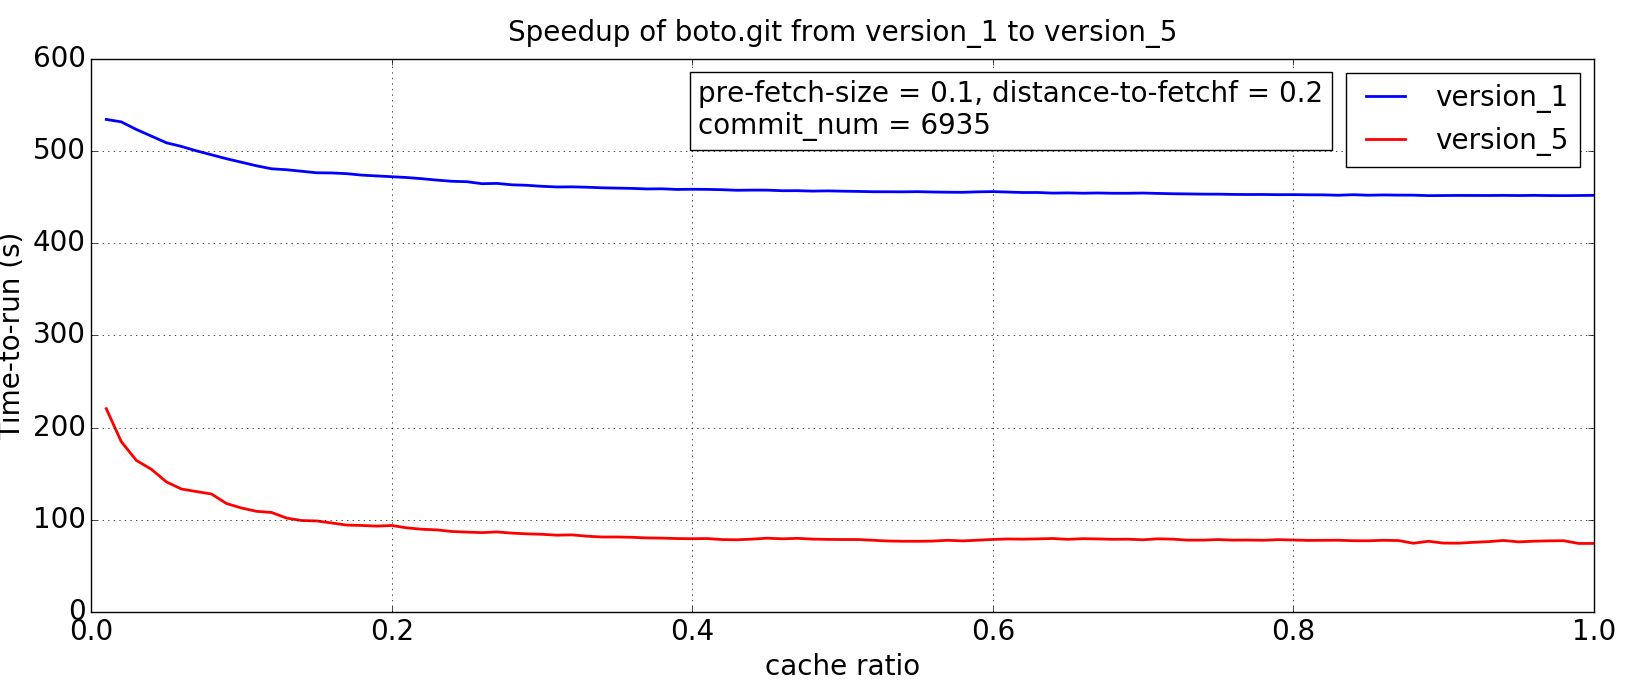
\includegraphics[width=1.0\textwidth]{speedup.png}

\caption{Speedup of boto.git and boto3.git between version\_1 and version\_5 with different cache-ratios}
\label{fig:speedup}
\end{figure}

We can see on figure \ref{fig:speedup} on the next page, how good is fast did it take for \fxch{} to run for a given cache-ratio. The figure is showing two versions: version\_1 (with sorting) and version\_5 (with ``select top $k$ from $n$''), and its clear that version\_5 is faster.
This speed-up is caused mainly by replacing sorting, as we will be using more linear operations (if $k >= n$) and $\mathcal{O}(n\log{k})$ operations, where for a single run $k$ is fix, and $n$ is changing.
\cleardoublepage
\chapter{Evaluation}
This chapter first introduces the repositories evaluated, and their properties. Then we will look at the results according to the evaluation method used by the original authors of \fxch{}. Finally, a new evaluation method is introduced, and two of the repositories are evaluated accordingly. 
\section{Repositories analysed and evaluated}
The algorithm was evaluated and analysed using five repositories: facebook-sdk.git\footnote{https://github.com/mobolic/facebook-sdk}, raspberryio.git\footnote{https://github.com/python/raspberryio}, boto3.git\footnote{https://github.com/boto/boto3}, boto.git\footnote{https://github.com/boto/boto} and django.git\footnote{https://github.com/django/django}. All these repositories were cloned, and \fxch{} was run on them locally: facebook-sdk.git was mainly used for testing purposes; raspberryio.git, boto3.git and boto.git was analysed completely; boto.git and django.git were used for performance evaluation. The repositories were chosen to have different number of commits, and to be mostly pure Python (except raspberryio.git which is only 43\% Python), also they have been used in earlier projects I was involved in, hence the idea to analyse them.
\clearpage
As all the repositories were cloned, the data presented here (such as the number of commits for a repository) resembles the data for the date when each repository was cloned, that is: 11-10-2015 for facebook-sdk.git; 22-04-2014 for raspberryio.git; 12-01-2016 for boto3.git; 18-01-2016 for boto.git; 28-03-2016 for django.git.
\section{Evaluation modules}
\subsection{Analysing \fxch{}}
To analyse and evaluate \fxch{} we need to run it several times each time with different parameters. The Analysis module contains different functions to perform different types of analysis. Out of the three key variables (cache-ratio, distance-to-fetch and pre-fetch-size) we fix one or two, and later we display the results found. The different analysis types implemented are listed below.
\subsubsection{\texttt{analyse\_by\_cache\_ratio}}Here, at a single analysis we fix both pre-fetch-size and distance-to-fetch, and run \fxch{} for 100 different cache sizes, that is cache-ratio $\in \{0.01, 0.02, 0.03 \dots 0.99, 1.00\}$. We run this for different pre-fetch-size and distance-to-fetch values, namely pre-fetch-size $\in \{0.1, 0.15, 0.2\}$ and distance-to-fetch $\in \{0.1, 0.2, 0.3, 0.4, 0.5\}$. That is, a complete analysis of this type will require $100*5*3=1500$ runs of \fxch{}.
\subsubsection{\texttt{analyse\_by\_fixed\_cache\_ratio}} 
Following the previous examples, here we fix the cache-ratio, and are interested in the best possible pre-fetch-size and distance-to-fetch for a given cache-ratio. We look at different cache-ratios, to be specific: $cache\_ratio \in \{0.05, 0.1, \dots 0.5\}$. 
\subsection{Displaying results}
We store all the results, for each analysis in .csv files. Once the .csv files were created, we read them and display the data using the matplotlib\footnote{http://matplotlib.org/} Python library. The Graph module is responsible for reading, and displaying the .csv files created by our Analysis module, as .png images using matplotlib.
\section{Evaluation over hit-rate}
\subsection{Results}
In the original paper \fxch{} was evaluated and analysed against hit-rate, that is the ratio of cache hits over all cache look-ups. It was found for several projects (such as Apache1.3, PostgreSQL, Mozilla and others in \cite{FixCache}) that hit-rate is between 0.65 and 0.95 for cache-ratio of 0.1, pre-fetch-size of 0.1 and distance-to-fetch of 0.5.
\begin{figure}[h]
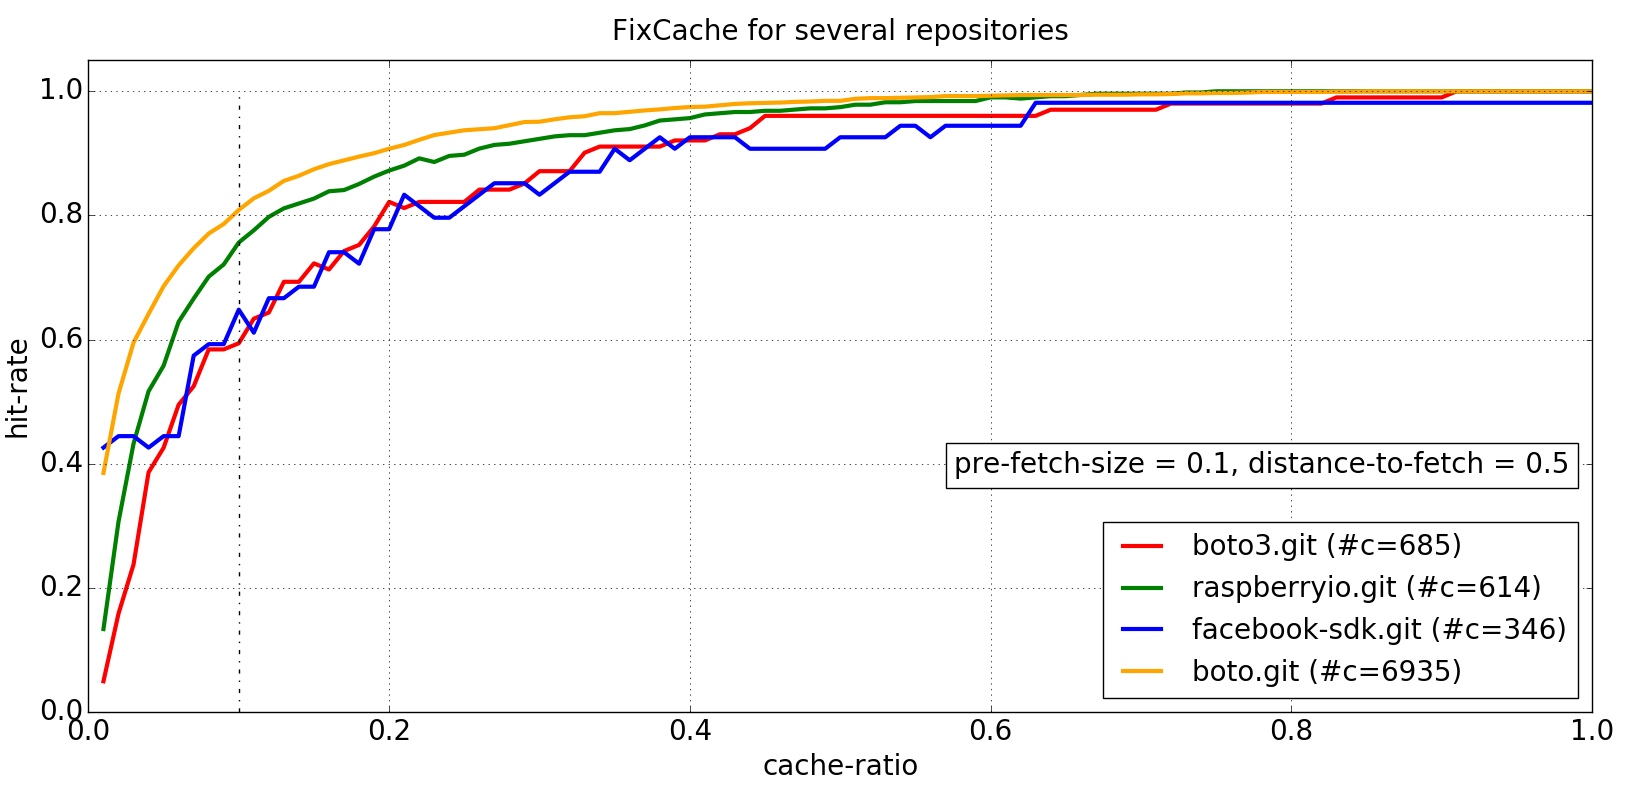
\includegraphics[width=1.0\textwidth]{plot_several.png}
\caption[Evaluation of \fxch{} according to hit-rate for different repositories.]{Evaluation of \fxch{} according to hit-rate for different repositories. Vertical dashed-line at cache-ratio of 0.1.}
\label{fig:v5_repos}
\end{figure}

For the same variables, similar results were found: hit-rate was always between 0.6 and 0.83, thus repositories analysed here performed slightly worse. Also, for repositories with higher number of commits we usually had a bigger hit-rate, as we can see in figure \ref{fig:v5_repos}. At cache-size of 0.2, we get an even better result of hit-rate which will be between 0.75 and 0.9. It seems that for bigger repositories (such as boto.git) the curve is smoother than for smaller ones, as one might expect.
\paragraph{What is the ``best'' cache-ratio?}From the figure \ref{fig:v5_repos} it can be deduced that for cache-ratio of 0.2 we already get a really good hit-rate, so 0.2 can be considered the ``best'' cache-ratio. For this ratio, for all possible distance-to-fetch and pre-fetch-size values the raspberryio.git has a hit-rate between 0.86 and 0.89, and boto.git has a hit rate between 0.9 and 0.92. Furthermore, if we fix pre-fetch-size and distance-to-fetch (0.1 and 0.5 respectively) all repositories looked at will have a hit-rate between 0.78 and 0.96. From this, it seems that we get a closer result to the original evaluation for a higher hit rate.

An interesting thing to note is that pre-fetch-size and distance-to-fetch does not change drastically our hit-rate as can be seen on the figure \ref{fig:fixed_cache}. This result was also found by Rahman \etal{}: they found that temporal locality has a significantly bigger impact on cache performance than new-entity-locality, changed-entity-locality (pre-fetch-size) and spatial locality (distance-to-fetch). That is, putting the most-recently faulty files to our contributes to our hit-rate the most from all \cite{Bugcache}.
\paragraph{Finding the best pre-fetch-size and distance-to-fetch}Even though pre-fetch-size and distance-to-fetch are not the highest predictors of the cache-performance, it is still worthwhile to look at which values of these variables is the hit-rate biggest.
\begin{figure}[h]
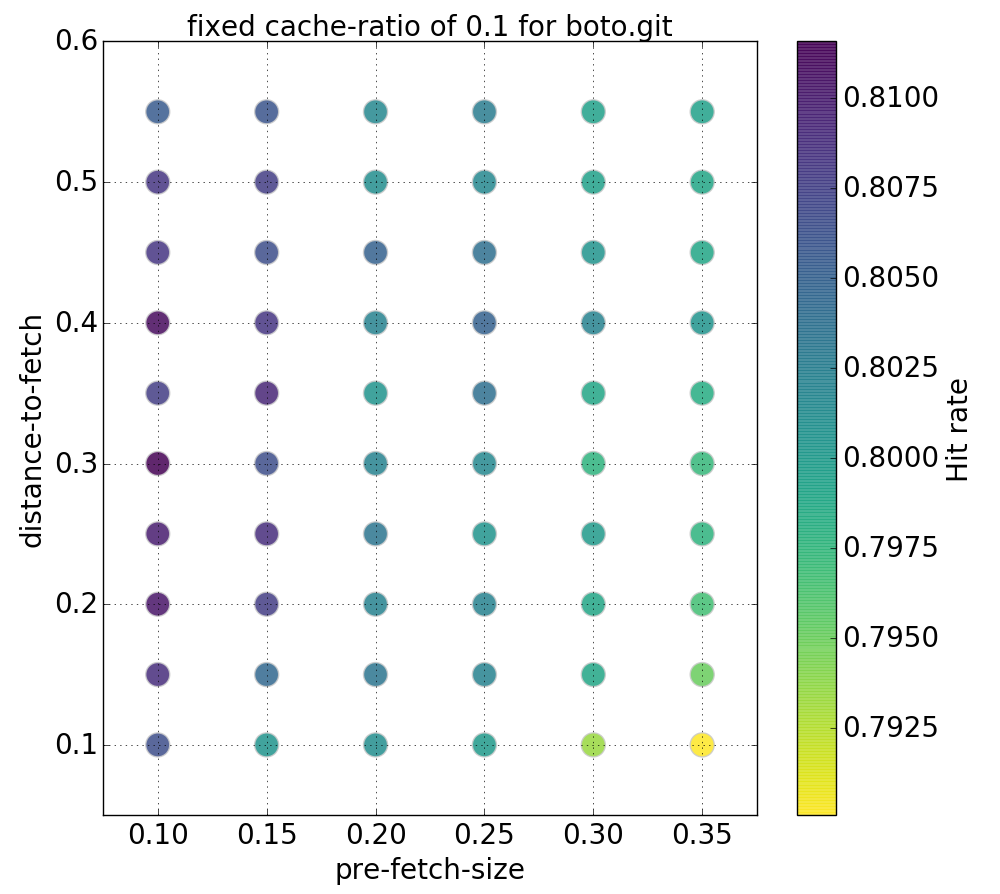
\includegraphics[width=0.5\textwidth]{fixed_cache-1.png}
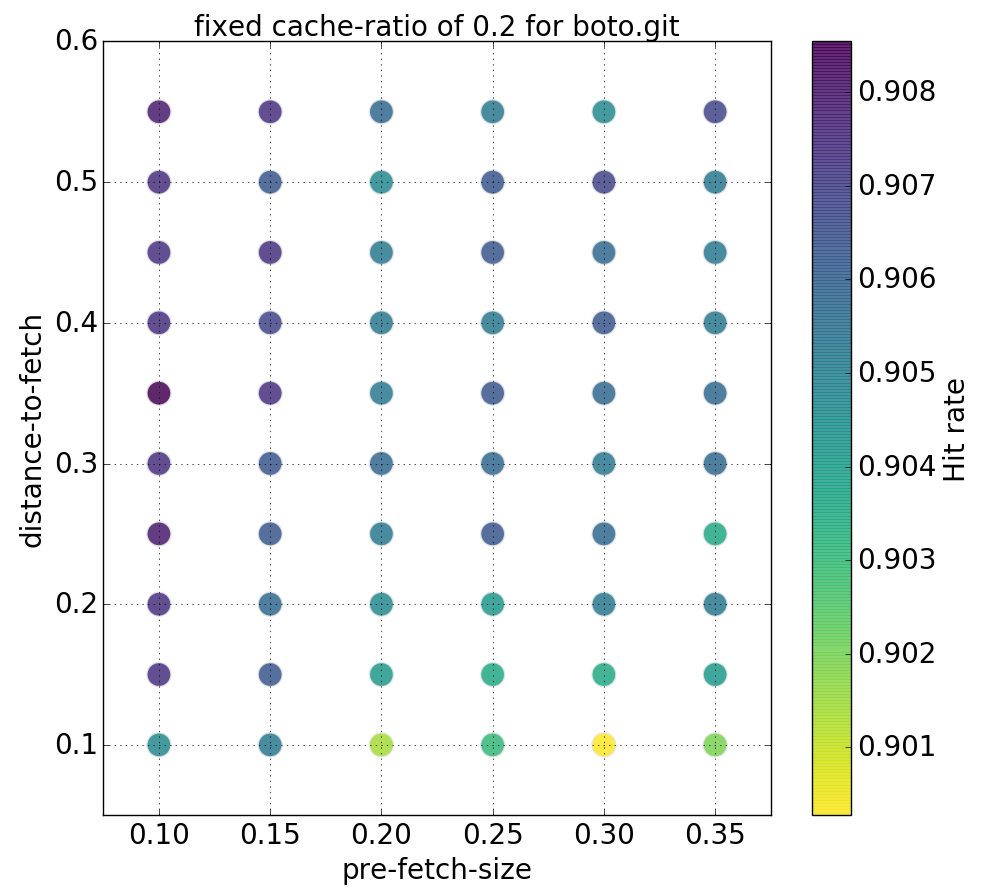
\includegraphics[width=0.5\textwidth]{fixed_cache-2.png}
\caption{Fixed cache-ratio analysis for boto.git}
\label{fig:fixed_cache}
\end{figure}
In figure \ref{fig:fixed_cache} we can see (for boto.git) the results of a fixed-cache-ratio analysis, where we fixed the cache-ratio to 0.1 and to 0.2. The results indicate that for both we will get the best results when pre-fetch-size is low and distance-to-fetch is either 0.3 or 0.4 or 0.5. These results are in line with what was found in previous implementations \cite{FixCache}.
\paragraph{Variance in hit-rate for different variables}How big is the difference between all the plots for a given repository, at any given cache-ratio?  Figure \ref{plot_all} shows all the analyses for facebook-sdk.git, boto3.git, raspberryio.git and boto.git. The figure itself does not plot each and every analysis (taking all pre-fetch-size and distance-to-fetch values it would mean 15 curves), rather it plots vertical bars for each cache-ratio, where the bottom of the bar starts at the lowest hit-rate and ends at the highest hit-rate from all the analyses. That is, the bars cover the area which would be touched by any of the 15 curves, and when a bar is taller, then the variance of hit-rates is also bigger at that cache-rate. As we can see boto3.git (which has a lot less commits than boto.git) has a higher variance in the hit-rate results, than boto.git. The biggest difference for boto3.git it will be 0.158 at cache-ratio of 0.12, for boto.git it will be 0.073 at cache-ratio of 0.02. Similarly the other two repositories with less commits than boto.git, raspberryio.git and facebook-sdk.git also have a high variance in this graph (with maximums of 0.076 at cache-ratio of 0.06 for raspberryio and 0.092 at cache-ratio of 0.16 for facebook-sdk), so we might deduce that the less commits a repository has, the bigger it's variance in the output will be.

\paragraph{What do these results mean?} When comparing with the original paper, the results are similar (0.65-0.95 vs 0.6-0.83), although the top hit-rate boundary (0.95 for 0.1 cache-ratio) was not achieved, the highest was 0.83 for boto.git. This top boundary is reached for the cache-ratio of 0.2, which might mean that this implementation works the same for bigger cache-ratios. It is important to note that when making such a comparison one does need to remember that this implementation differs from the original in two key things: firstly, it was implemented for Git rather than Subversion and CSV and secondly it was run on open-source Python repositories rather than on C/C++ or Java projects. 
\clearpage
\begin{figure}[t]
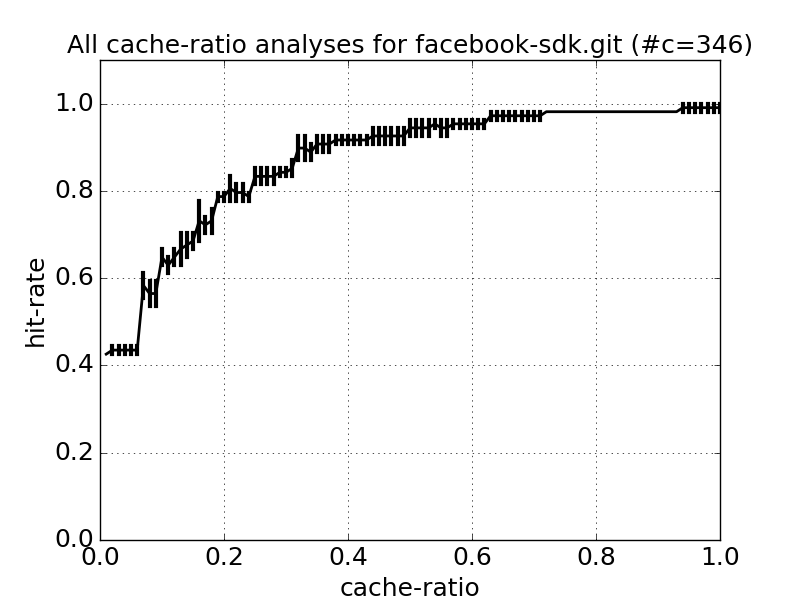
\includegraphics[width=0.5\textwidth]{plot_all-facebook-sdk.png}
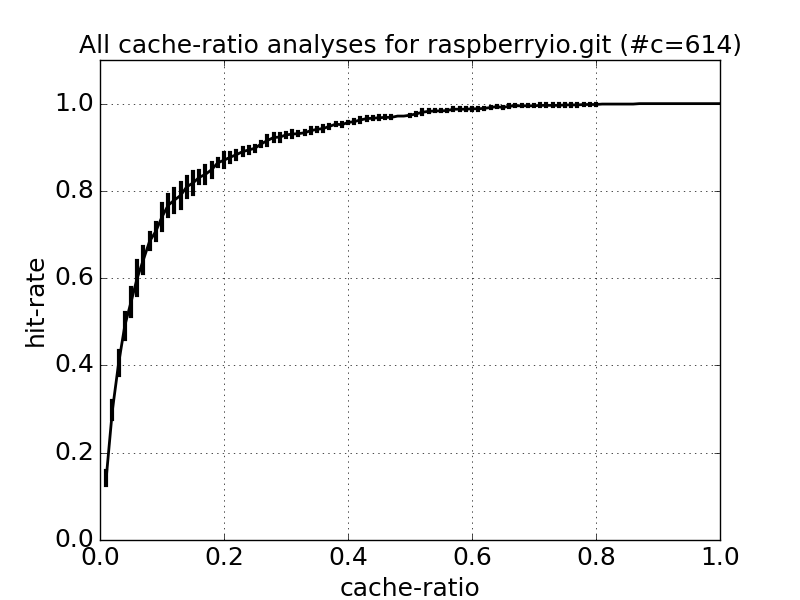
\includegraphics[width=0.5\textwidth]{plot_all-raspberryio.png}
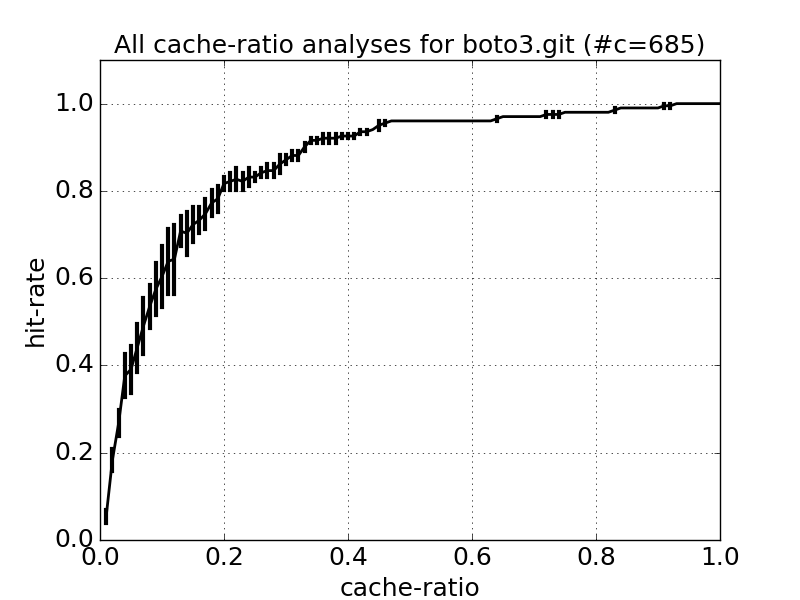
\includegraphics[width=0.5\textwidth]{plot_all-boto3.png}
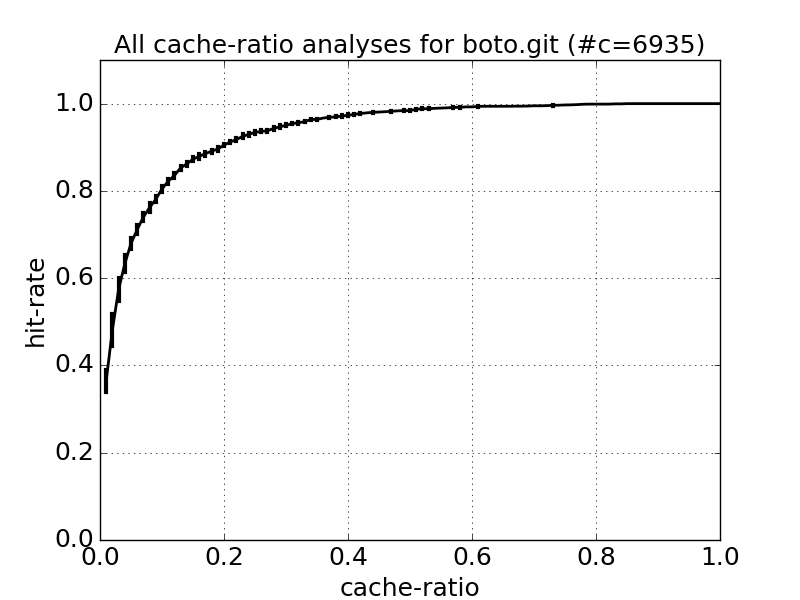
\includegraphics[width=0.5\textwidth]{plot_all-boto.png}
\caption{Showing all cache-ratio analyses for facebook-sdk.git, raspberryio.git, boto3.git and boto.git.}
\label{plot_all}
\end{figure}
From these results, the following points could be stated:
\begin{enumerate}
\item For a given repository $R$, the relationship between the number of faulty files in R and the size of $R$ is not linear, as for a bigger $R$ the variance decreases with variables staying the same (percentage of $R$'s size).
\item The results found do not differ significantly from the results found in the original paper, although the same boundaries are reached for a higher cache-ratio of 0.2. Other than that, the variance between the hit-rates of different repositories is also quite big for cache-ratio of 0.1 (0.6-0.83 vs. 0.65-0.95 in the original paper), and this result seems to be connected to the number of commits in a repository (that is the history of a repository).
\clearpage
\item There might be several possible explanations for these differences in cache-ratios:
\begin{enumerate}
\item Python programmers make more mistakes (as opposed to C/C++ or Java developers) as the language is structured differently (ex. loose type-system: duck-typing; possibly several others), so in general Python repositories are more vulnerable.
\item Open-source projects are more bug-prone as they are less ``looked-after'' and the development process is more chaotic than in well-organised companies and teams.
\item As Git is a distributed, de-centralized version control system, programming with the help of Git might be less structured and organised than programming with the help of Subversion or other centralised systems.

Further analysis of these differences was out of the scope of this dissertation, but they definitely would be interesting to investigate further.
\end{enumerate}
\item From these results we can see that \fxch{} works for Git, and also it works for open-source Python repositories, however the hit-rate for the same parameters was found to be slightly lower on-average.
\end{enumerate}
\subsection{Criticism}
Authors of \fxch{} claimed that after running the algorithm, our cache will contain the files which ``are most likely to have a bug in the future''. However, they did not specify what this ``future'' is, how many commits/days/weeks ahead does \fxch{} predict? To investigate this, the notion of `windowed-repository evaluation'  was introduced (which will be explained later, on page \pageref{windowedrep} ). Using this technique it was found that \fxch{} works for the first few commits in the future, but later it's accuracy drops.

Another criticism is that \fxch{} treats files as atomic entities whereas this is hardly the case. Files have several metrics on which they differ, such as LOC, or code density. If our algorithm identifies say 10\% of our file base, this 10\% might account for 20\% of all lines in the repository. This will be generally the case, as longer files are expected to have more impact and importance on our project, hence they'll have more bugs. Sadowski and colleagues found that even if this is the case, \fxch{} finds the files with the highest ``defect densities'' (files which are more bug dense: LOC/\#bugs), so the algorithm is still helpful \cite{Bugcache}.

\section{How good is \fxch{}?}\label{windowedrep}
Evaluating over hit-rate leaves several questions open, for example ``Is \fxch{} identifying files which truly have bugs in the future?'', ``For how many commits in the future will \fxch{} work?''. When trying to answer these questions the notion of a `windowed-repository' was created. This means, that rather than running \fxch{} for all commits until now, we divide the commit history to a window and a horizon, and run \fxch{} on the window and we check on the horizon whether it actually worked. That is, say our window is of size 0.9, our horizon then is 0.1, and say we have 1000 commits. If this is the set-up, then we would run \fxch{} on the first 900 commits, and then check the following 100 whether it actually worked. If we look at figure \ref{window_horizon}, t0 would be at commit \#1 and tNow would be at commit \#1000. At each point in our timeline below, $C_{tX} = floor(tX)$, as the time axis below corresponds to the commit order from commit 1, to the latest commit.

\begin{figure}[h]
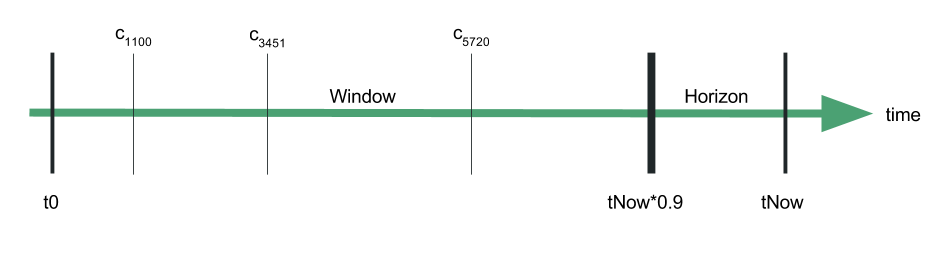
\includegraphics[width=1.0\textwidth]{window_horizon.png}

\caption{Window and horizon presented on a timeline of commits}
\label{window_horizon}
\end{figure}

\subsection{Methodology}
As mentioned before, we run \fxch{} for each repository, but we stop at tNow*0.9 number of commits (the window). By default when performing such an evaluation (using \texttt{evaluation} module's \texttt{evaluate\_repository} method) our default parameters are: window-ratio of 0.9, cache-ratio of 0.1, pre-fetch-size of 0.1 and distance-to-fetch of 0.5.

At the time we stop, we have some files in our cache, and this cache would be left unchanged as we walk through our horizon, lets call the set of files in the cache $CH$. Let tHStart = tNow*0.9, then at each point tX in our horizon (that is $\forall c_{tX} \in \{c_{tHStart}, \dots, c_{tNow}\}$ we can define the following two sets:
\begin{itemize}
\item Normal-file-set at tX: Files which were changed (committed) between tHStart and tX, but were not part of a bug-fixing commit in this interval. Lets call this set $NF$.
\item Faulty-file-set at tX: Files which changed in the same interval (as above), but they were at least once changed as a part of a bug-fixing commit. Lets call this set $FF$.
\end{itemize}

From this, we can define the following properties:
\begin{itemize}
\item True-positives at tX ($TP$): The files in our cache, which indeed were faulty in [tHStart:tX]. That is $TP = FF \cap CH$.
\item False-positives at tX ($FP$): The files in our cache, which were not faulty in [tHStart:tX]. That is $FP = NF \cap CH$.
\item True-negatives at tX ($TN$): The files which are in our Normal-file-set in [tHStart:tX], and are not in our cache. That is $TN = NF \setminus CH$.
\item False-negatives at tX($FN$): The files which are in our False-file-set in [tHStart:tX], and are not in our cache. That is $FN = FF \setminus CH$.
\end{itemize}
From this we can see that all changed files in [tHStart:tX] are equal to $TP \cup FP \cup TN \cup FN$, and also that these sets are distinct.
\paragraph{Performance metrics}Following the definition of $TP$, $TN$, $FP$ and $FN$ we can define several performance metrics on which we will evaluate our windowed-repositories\cite{IR}:
\begin{enumerate}[label=(\alph*)]
\item Precision: $\frac{|TP|}{|TP| + |FP|}$
\item False discovery rate: $\frac{|FP|}{|TP| + |FP|}$
\item Negative predictive value: $\frac{|TN|}{|TN| + |FN|}$
\item False omission rate: $\frac{|FN|}{|TN| + |FN|}$
\item Recall (or Sensitivity): $\frac{|TP|}{|TP| + |FN|}$ 
\item Specificity: $\frac{|TN|}{|TN| + |FP|}$
\item Accuracy: $\frac{|TP| + |TN|}{|TP| + |FP| + |TN| + |FN|}$
\item F\textsubscript{$\beta$} score: \[(1+\beta^2)*\frac{precision*recall}{(\beta^2*precision)+recall} = \frac{(1+\beta^2)*|TP|}{(1+\beta^2)*|TP| + \beta^2*|FN| + |FP|}\]

Where $\beta$ specifies whether we weight precision or recall higher.
\end{enumerate}
\subsection{Precision, recall and F\textsubscript{2} score}
\begin{figure}[h]
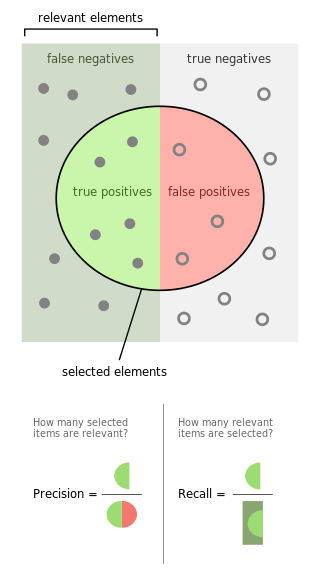
\includegraphics[width=0.5\textwidth]{Precisionrecall.png}
\centering
 \begin{minipage}{\linewidth}
    \caption[Precision and recall.]%
    {Precision and recall. Figure taken from Wikipedia\footnotemark.}
    
  \end{minipage}

\end{figure}
\footnotetext{https://en.wikipedia.org/wiki/Precision\_and\_recall}
Out of the metrics above, we are mostly interested in precision, recall and F\textsubscript{2} score at each bug-fixing commit in our horizon. Figure 4.5 shows these metrics in a Venn-diagram. In this diagram the \textit{relevant elements} corresponds to fixed-files (that is ones with bugs) whereas \textit{selected elements} corresponds to files in our cache. Following this, we can define precision as the ratio of \textit{selected and relevant} files and \textit{selected but not relevant} files and recall as the ratio of \textit{selected and relevant} files and \textit{relevant} files. That is precision is tells us the percentage of files in the cache which are indeed buggy at each bug-fixing commit in our horizon while recall tells us the percentage of correctly predicted buggy files. 

As defined above the F\textsubscript{$\beta$} score weight precision and recall according to the parameter $\beta$. Since \fxch{} supposed to identify files which are ``most likely to contain a bug in the future'' recall should be weighted higher, as when finding buggy files it should be more important to correctly identify the biggest subset of truly faulty files than to have some false-positives, therefore F\textsubscript{2} score will be used for evaluation. After substituting 2 for $\beta$ we get that:
\[
	F_2 = \frac{5 * precision * recall}{4 * precision + recall} = \frac{5 * |TP|}{5 * |TP| + 4 * |FN| + |FP|}
\]
\clearpage
\subsection{Results}
\subsubsection{Evaluating boto.git}
\begin{figure}[ht!]
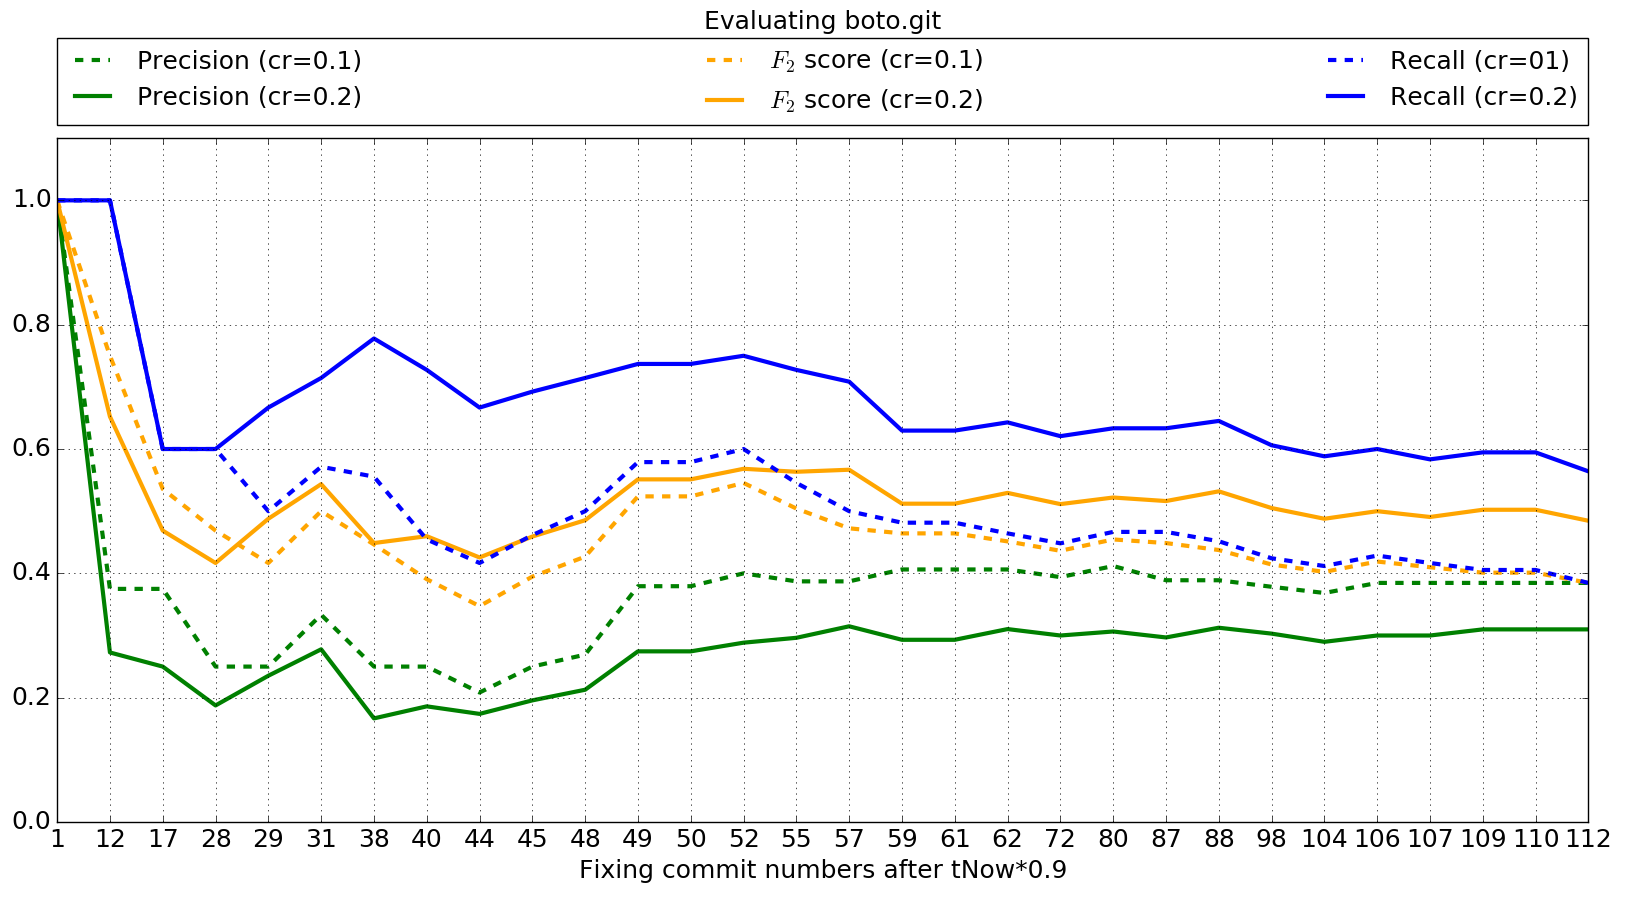
\includegraphics[width=1.0\textwidth]{evaluating_boto.png}
\caption[Evaluating boto.git: recall, precision and $F_2$ score]{Evaluating boto.git with precision, recall and F\textsubscript{2} score for the first 30 commits in the horizon after tNow*0.9. Here cr means cache-ratio.}
\label{evaluating_boto}
\end{figure}
Figure \ref{evaluating_boto} shows precision, $F_2$ score and recall for the first 30 fixing commit in the horizon for boto.git (at cache-ratio of 0.1 and 0.2), which at the time of evaluation has 6935 commits. For cache-ratio of 0.2 we can see that for the first fixing-commit in the horizon (that is for $C_1$) all the metrics are equal to 1.0. That is our algorithm identified buggy files fixed at $C_1$ correctly. However, at the second fixing commit, there is a massive drop in all three metrics, except for recall, when this drop occurs between $C_{12}$ and $C_{17}$ rather than between $C_1$ and $C_{12}$. If we look at recall, it always stays above 0.6 (except for the last few commits), that is we will identify at least 60\% of the truly buggy files. Furthermore, after the sudden drop, it will have it's peak of 0.78 at $C_{38}$, after which it will continue to drop.

Recall at cache-ratio of 0.1 is lower or equal to the recall at 0.2, which is expected. However, precision is higher, which is due to the higher number of false-positives identified when having a bigger cache.

From this figure, we can deduce that for boto.git \fxch{} does only perform well for the first two commits in terms of recall, and does poorly afterwards (except the peak at $C_{38}$); similarly it only works for the first commit for the other two metrics, after which precision and $F_2$ score will also drop. This means that in this case \fxch{} should not be used as a long-term bug prediction technique, but rather as a source for finding recently introduced bugs. Also, we can see that the performance is better with cache-ratio of 0.2.
\subsubsection{Evaluating django.git}
\begin{figure}[ht!]
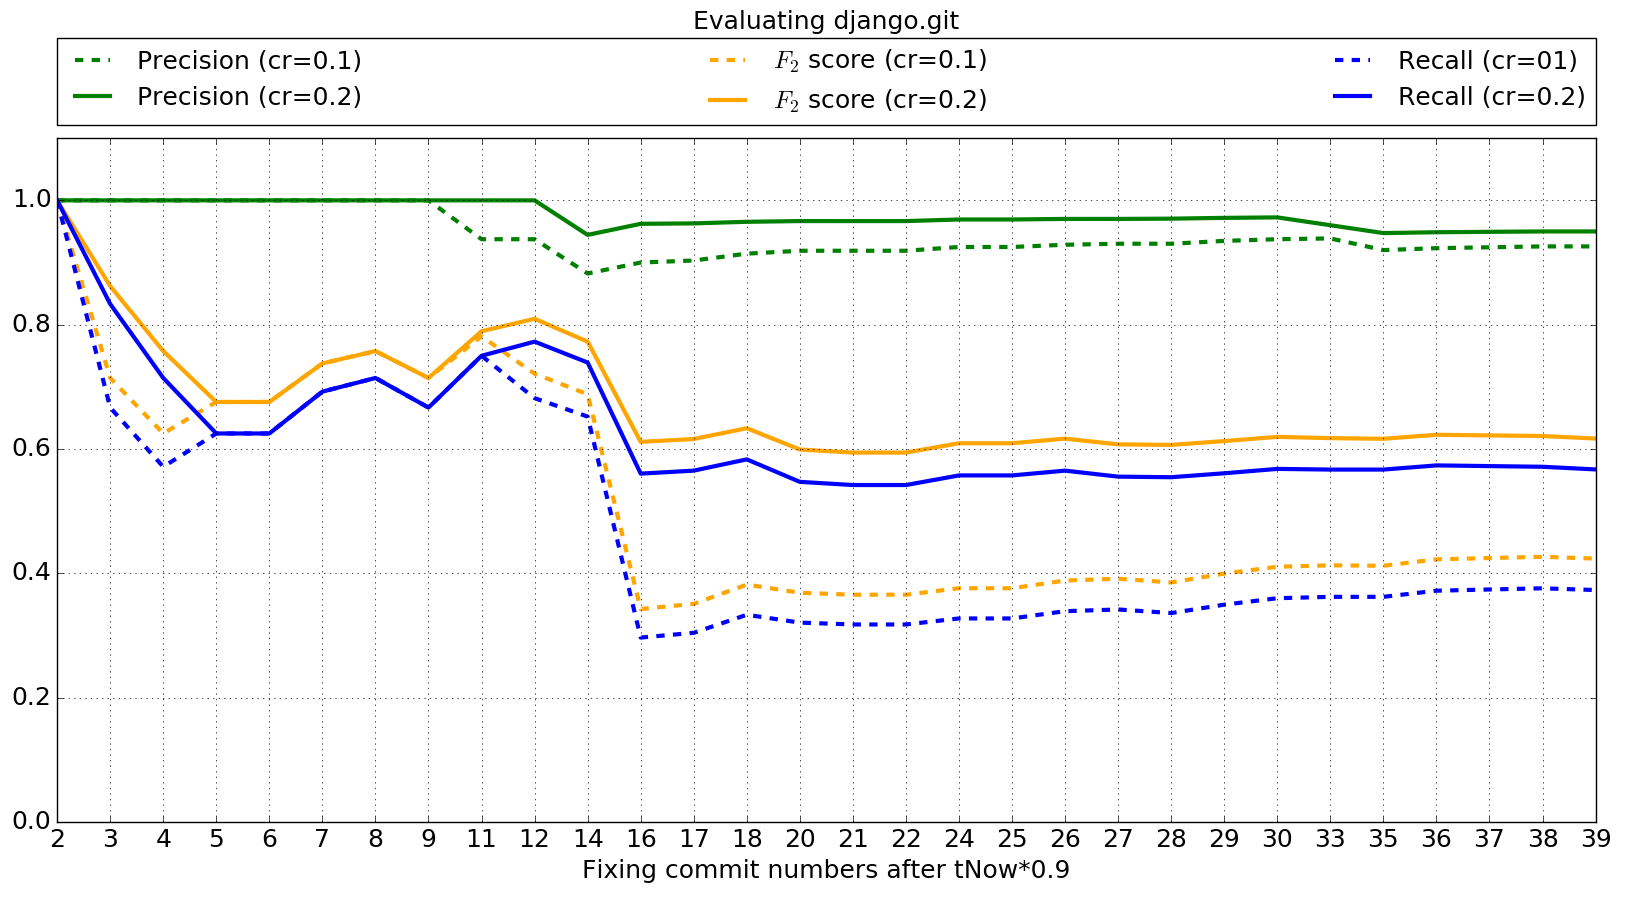
\includegraphics[width=1.0\textwidth]{evaluating_django.png}
\caption[Evaluating django.git: recall, precision and $F_2$ score]{Evaluating django.git with precision, recall and F\textsubscript{2} score for the first 30 commits in the horizon after tNow*0.9. Here cr means cache-ratio.}
\label{evaluating_django}
\end{figure}
Figure \ref{evaluating_django} shows the same data as \ref{evaluating_boto} but this time for django.git, which has 22352 commits at the time of the evaluation. Also, a difference to observe is that nearly every commit in the horizon looked at is a fixing-commit (as we arrive at commit \#39 which is the 30\textsuperscript{th} fixing-commit), that is fixes occur much more frequently. This is likely due to the fact that django.git is already a complete product, and all these fixing-commits are responses to issues reported by users rather than by the developers themselves\footnote{This was deduced by manually going through the commit history of django.git and reading (and understanding) the context of these fixing commits, and why are fixing commits so frequent.}. That is the implementation of django.git is finished (at least on the master branch) and hence nearly all the commits are fixing ones. 

Again as with figure \ref{evaluating_boto} the metrics are higher for cache-ratio of 0.2 (even for precision this time). However, the difference between cache-ratios is much bigger for the $F_2$ score after the drop happens (here at $C_{12}$). We can see that the difference between $F_2$ scores for cache-ratio of 0.1 and 0.2 will be at least 0.2 after this point. This difference was never as dramatic in figure \ref{evaluating_boto}.

Another key difference between this figure and figure \ref{evaluating_boto}: precision stays high for all the commits. That is, if a file is identified as a buggy-file here, it is likely to indeed be buggy: our cache indeed has faulty files in it. Other than this, recall also drops after the first two commits, after which it also climbs back to a peak at around 0.78 (here at $C_{12}$), and after this peak it will drop below 0.6, so it is slightly worse than recall for boto.git.
\section{Summary}
When evaluating our repositories over hit-rate similar results were found to those of the original paper, however generally they were slightly lower on-average for cache-ratio of 0.1. For cache-ratio of 0.2 the results resembled more the findings of Kim \etal{} for their 10\% cache-size \cite{FixCache}.

The parameters (for a fixed cache-ratio) for which we have the best hit-rate possible were also found to be close to the ones identified in the original paper.

With the new evaluation technique, it has been found that \fxch{} as a predictor only performs well for the first few commits in the horizon (future) after which it's performance drops.
\cleardoublepage
\chapter{Conclusion}
\section{Summary of work}
This dissertation presents an implementation of \fxch{}, an algorithm which from a repository's commit-history identifies a subset of files which are most likely to have a bug in the future. The algorithm was implemented in Python for Python repositories on GitHub. 

Apart from implementing \fxch{}, it was also explored how Git can be used for repository analysis, specifically for \fxch{}, and how any pitfalls related to this approach should be tackled. Overall, the project goals outlined in the project proposal were met, and all the components were completed on schedule. 

The algorithm was evaluated against open-source Python repositories publicly accessible via GitHub. It was found that these repositories perform slightly poorer in terms of \fxch{'s} hit-rate when compared to the repositories evaluated by Kim \etal{} \cite{FixCache}. It is yet to be discovered whether this difference is due to to Python itself, or the fact that this dissertation only looked at open-source public Git repositories.

\clearpage
\section{Novel Contributions}
Most of the previous implementations were implemented using Subversion or CVS as their back-end Version Control System \cite{FixCache}\cite{Sadowski}, only Rahman \etal{} used Git (repositories from GitHub) before \cite{Bugcache}. None of these implementations however were evaluated on Python repositories, all of them used C/C++ and Java projects, so evaluating the algorithm on Python is a novelty of this dissertation.

Another contribution was the introduction of the `windowed-repository evaluation'. It has been found that using this evaluation paradigm (that is in terms of precision, recall and F\textsubscript{2} score) \fxch{} only performs highly for the first few commits in the future, later it's performance drops (except precision for django.git). This means, that \fxch{} should only be used for immediate predictions, as it's performance drops in the long-term, so it should be re-run after each bug-fixing commit to always have an up-to-date prediction.
\section{Limitations and future work}
A limitation of this \fxch{} implementation is that it is quite heavy-weight: for over 22 thousand commits of django.git, one run required up-to 3 hours to complete, so for large projects it might not be a feasible solution for bug prediction. This limitation however might only be due to the fact that this version was implemented in Python, which is considered to be slower than other highly used languages as Java or C/C++.

Further work could be done in achieving a faster implementation, to make it usable for larger repositories with several tens-of-thousands of commits.

Also, a major improvement in terms of hit-rate could be the implementation of a more sophisticated per line analysis of lines `which truly contribute to a bug' (following the methods proposed by Kim \etal{} \cite{KimZim}).

Finally, it would be also interesting to implement a method-level \fxch{} for Git, in order to compare the results with the method-level results found by Kim \etal{} \cite{FixCache}.

\addcontentsline{toc}{chapter}{Bibliography}
\bibliography{refs}
\cleardoublepage
\appendix
\chapter{Modules}

\definecolor{backcolour}{rgb}{0.95,0.95,0.92}
\section{\texttt{filemanagement.File} class}
\lstinputlisting[language=Python,backgroundcolor=\color{backcolour},keywordstyle=\color{blue},breaklines=true,
firstline=49,lastline=148, showspaces=false,showstringspaces=false, numbers=left]{../fixcache/filemanagement.py}
\clearpage
\section{\texttt{filemanagement.Distance} class}
\lstinputlisting[language=Python,backgroundcolor=\color{backcolour},keywordstyle=\color{blue},breaklines=true,
firstline=242,lastline=319, showspaces=false,showstringspaces=false, numbers=left]{../fixcache/filemanagement.py}
\clearpage
\section{\texttt{cache} module}
\lstinputlisting[language=Python,backgroundcolor=\color{backcolour},keywordstyle=\color{blue},breaklines=true, showspaces=false,showstringspaces=false, numbers=left]{../fixcache/cache.py}
\chapter{Project Proposal}
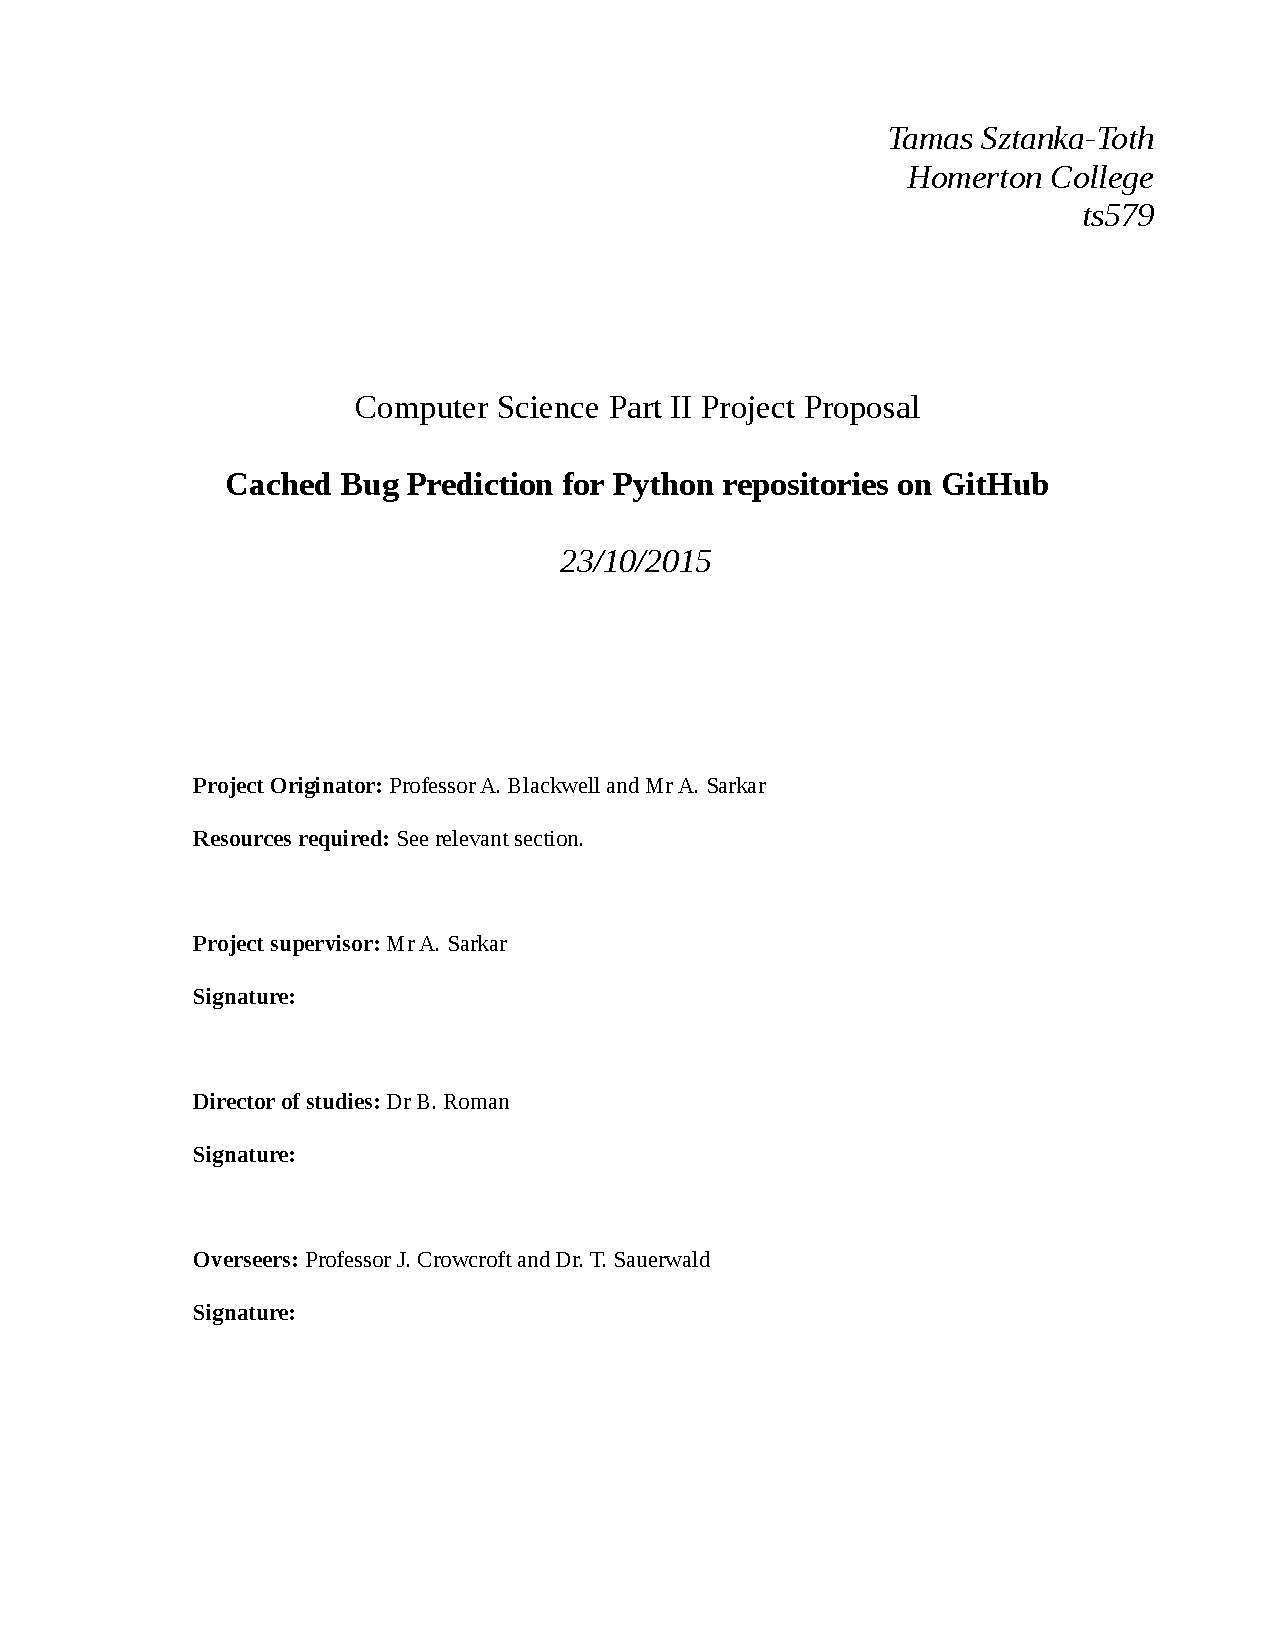
\includepdf[pages=-]{proposal_final.pdf}


\end{document}
